\documentclass[11pt,a4paper]{article}

% Encoding and fonts
\usepackage[utf8]{inputenc}
\usepackage[T1]{fontenc}
\usepackage{lmodern}

% Layout and typography
\usepackage[a4paper, margin=1in]{geometry}
\usepackage{microtype}
\usepackage{setspace}
\setstretch{1.1}
\setlength{\parskip}{0.45em}
\setlength{\parindent}{0pt}
\setlength{\emergencystretch}{3em}
\clubpenalty=10000
\widowpenalty=10000
\displaywidowpenalty=10000

% Math
\usepackage{mathtools}
\usepackage{amssymb}

% Graphics and floats
\usepackage{graphicx}
\usepackage{float}
\usepackage[section]{placeins}
\usepackage[font=small,labelfont=bf,format=hang]{caption}
\usepackage{subcaption}
\captionsetup{width=0.94\linewidth}
\graphicspath{{figures/}}

% Tables
\usepackage{booktabs}
\usepackage{array}
\usepackage{longtable}
\newcounter{none}
\usepackage{calc}
\usepackage{etoolbox}
\makeatletter
\patchcmd\longtable{\par}{\if@noskipsec\mbox{}\fi\par}{}{}
\makeatother
\IfFileExists{footnotehyper.sty}{\usepackage{footnotehyper}}{\usepackage{footnote}}
\makesavenoteenv{longtable}
\usepackage{multirow}
\renewcommand{\arraystretch}{1.08}

% Lists
\usepackage{enumitem}
\setlist{topsep=0.35em,itemsep=0.15em,parsep=0pt,partopsep=0pt}

% Page style
\usepackage{fancyhdr}
\setlength{\headheight}{14pt}
\pagestyle{fancy}
\fancyhf{}
\fancyfoot[C]{\thepage}
\fancyhead[L]{\footnotesize\itshape Brent Baumgartner and Edmundo Lopez-Sola}
\fancyhead[R]{\footnotesize\itshape Self-Energy and Witnessing}
\renewcommand{\headrulewidth}{0.2pt}

% Colors and links
\usepackage{xcolor}
\definecolor{linkblue}{RGB}{0,51,153}
\usepackage{hyperref}
\hypersetup{
  colorlinks=true,
  linkcolor=linkblue,
  citecolor=linkblue,
  urlcolor=linkblue,
  pdftitle={Self-Energy, Witnessing, and the Revision of Part Beliefs}
}
\usepackage{cleveref}
\crefname{figure}{Fig.}{Figs.}
\crefname{table}{Table}{Tables}
\crefname{section}{Sec.}{Secs.}
\crefname{equation}{Eq.}{Eqs.}

\providecommand{\tightlist}{%
  \setlength{\itemsep}{0pt}\setlength{\parskip}{0pt}}

% Pandoc 3.x compatibility: \pandocbounded constrains image width to \textwidth
% Uses \resizebox to scale down oversized images while preserving aspect ratio
\newcommand{\pandocbounded}[1]{%
  \setbox0=\hbox{#1}%
  \ifdim\wd0>\textwidth
    \resizebox{\textwidth}{!}{#1}%
  \else
    #1%
  \fi
}

\makeatletter
\renewcommand{\maketitle}{
  \thispagestyle{empty}
  \begin{center}
    {\LARGE\bfseries \@title\par}
    \vspace{0.55em}
    {\large \@author\par}
    \vspace{1.4em}
  \end{center}
}
\renewcommand\section{\@startsection{section}{1}{0pt}{2.3ex plus 0.6ex minus 0.2ex}{1.1ex plus 0.2ex}{\large\bfseries}}
\renewcommand\subsection{\@startsection{subsection}{2}{0pt}{1.8ex plus 0.5ex minus 0.2ex}{0.8ex plus 0.2ex}{\normalsize\bfseries}}
\renewcommand\subsubsection{\@startsection{subsubsection}{3}{0pt}{1.4ex plus 0.4ex minus 0.2ex}{0.6ex plus 0.2ex}{\normalsize\itshape}}
\makeatother

\title{\textbf{Self-Energy, Witnessing, and the Revision of Part
Beliefs}\\[0.4em]\large An Active Inference Account of Internal Family
Systems}
\author{Brent Baumgartner and Edmundo Lopez-Sola}
\date{}

\begin{document}
\maketitle

\section*{Abstract}

Sometimes \emph{I am afraid.} Sometimes \emph{a part of me is afraid.}
Same activation, different relationship. Internal Family Systems treats
that distinction as clinically decisive. This paper asks how to state it
in computational terms without flattening what the clinical method is
actually doing.

We propose a minimal active inference account of that distinction. In
IFS terms, parts are burdened inner beings with characteristic fears,
roles, and trust conditions; change occurs when a part can be witnessed
from Self rather than blended with. In the present model, that clinical
picture is operationalized as learned local control models within a
single generative model: bundles of priors over self-state, world-state,
policy, and expected outcome. The key variable is \textbf{Self-energy}
--- used here as a composite of autonomic-social regulation and
metacognitive depth --- which determines whether part activation
produces \textbf{blending} or \textbf{witnessing}. In blending, the part
captures inference: its beliefs feel like identity and present context
loses inferential force. In witnessing, the same part remains active
while present-context evidence stays online, so its beliefs can be held
as object rather than lived as the whole subject.

The simulations support three claims. First, matched activation does not
guarantee matched learning: exposure-like contact and witnessing-like
contact diverge when Self-energy changes the precision balance between
part priors and present evidence. Second, under the self-state-upstream
architecture (H1), witnessing revises self-state before threat meaning,
and threat meaning before protective policy. Third, the model
distinguishes witnessing from both indiscriminate calm and dissociative
quiet: adaptive fear remains in real danger, while dissociation reduces
distress without revising upstream priors. Companion simulations show
that part formation depends strongly on threat under low control, and
that multi-part polarization can be modeled as mutual threat attribution
between incompatible local control regimes.

The account is deliberately minimal. It does not yet formalize full
protector negotiation, therapist-client dyadic regulation, or self-like
parts. The claim is narrower than that: the therapeutic distinction in
IFS between \emph{being} a part and \emph{being with} a part can be
stated as a difference in inferential regime, and that difference goes a
long way toward explaining why some activations merely repeat the past
while others revise it.

\section{Introduction}\label{introduction}

Sometimes \emph{I am afraid.} Sometimes \emph{a part of me is afraid.}
Same activation, different relationship.

Consider a simple case. A person who was badly frightened by a dog as a
child sees an off-leash dog running toward them in a park. Their chest
tightens. Their body pulls back. One organization of the system becomes
certain all at once: \emph{dogs are dangerous; I am small; get away
now.} In ordinary fear-learning language, that looks like a threat
response. In IFS, it is described more specifically. A burdened part is
active, protectors are organizing around it, and the central question is
whether the person is now blended with that part or can remain with it.

That distinction is ordinary in IFS practice and underdescribed in most
formal accounts. If the activation takes over, the fear is not
experienced as one perspective among others; it becomes reality. The dog
is dangerous now. The body is small now. Avoidance feels necessary now.
If the same activation remains present while also being held in
awareness, the fear is still there, but the system is no longer speaking
only from inside the part. The person can relate to it.

IFS treats that relational difference as load-bearing. The therapist
does not simply increase contact with the dog, the memory, or the feared
affect. The therapist helps the client unblend from the activated part,
approach it from Self, and remain in relationship to it long enough for
something new to happen. That is why the method keeps returning to
questions like: \emph{How do you feel toward this part?} \emph{What does
it fear would happen if it stopped?} \emph{Will it let you get closer?}
The intervention is not organized around activation alone. It is
organized around who is relating to whom inside the system.

The claim of this paper is direct. The decisive therapeutic variable is
not activation alone. It is the relation of the system to activated
part-content. We propose that this relation is formalizable, tractable,
and clinically consequential. The governing variable in the present
account is \textbf{Self-energy}.

This paper is not arguing that IFS replaces exposure, schema work, or
other evidence-based approaches. The claim is narrower. Different
therapies alter different inferential variables. Exposure changes what
the system learns under contact with feared stimuli. IFS, at its core,
changes whether the activated part takes over or can be held in context.
Before translating that claim into active inference, it helps to state
the clinical picture in IFS's own terms.

The rest of the paper is straightforward. Section 2 explains the
phenomenon in IFS language. Section 3 turns that account into a
computational translation and introduces only the active inference
machinery the argument needs. Sections 4--6 define parts formally, show
how they form, and explain how they persist. Sections 7--9 formalize
Self, Self-energy, blending, witnessing, and the conditions under which
only witnessing supports durable revision. Sections 10--11 sketch
protectors and polarization. Sections 12--13 present the simulations and
results. Section 14 closes with what the model explains, where it is
still thin, and what should come next.

\section{IFS in Its Own Terms}\label{ifs-in-its-own-terms}

IFS begins from a simple claim: the mind is multiple, and that
multiplicity is organized. People have parts. Some parts carry terror,
shame, grief, helplessness, or loneliness. These are often called
\emph{exiles} because the system keeps them out of ordinary
consciousness when their pain would be too much. Other parts work to
prevent that activation. These are \emph{protectors}. Some are
\emph{managers}: they anticipate trouble, control situations, avoid
risk, and keep life organized so the exile does not break through.
Others are \emph{firefighters}: they react after activation has already
begun and try to shut it down fast, often through dissociation, numbing,
rage, or impulsive action.

IFS also posits \textbf{Self}. Self is not another part with better
ideas. It is the state in which the person is not captured by any one
part and can relate with curiosity, calm, compassion, and clarity. In
practice, therapists use Self as both a diagnostic and a therapeutic
reality. If the client can feel warmth, respect, or curiosity toward an
activated part, there is enough Self-energy in the system to proceed. If
the client says \emph{I hate this scared part} or \emph{I need it gone},
the therapist assumes another protector is now blended and works there
first.

The dog example makes the structure concrete. A child is bitten,
cornered, or badly frightened by a dog. An exile comes to carry terror
and helplessness. A manager learns to scan sidewalks, cross the street,
and keep distance before the fear surges. If a dog gets too close
anyway, a firefighter may take over with panic, collapse, dissociation,
or an urgent need to flee. From the inside, the episode does not feel
like a neutral memory being retrieved. It feels immediate: \emph{this
dog is dangerous; I am small; I have to get away}.

In IFS, the therapeutic question is therefore not just whether the fear
has been activated. It is whether the person is \textbf{blended} with
the part or can become \textbf{unblended} enough to relate to it.
Blending means the part is speaking as the whole person. Unblending
means the person can speak \emph{for} the part rather than only
\emph{from} it. The linguistic difference is small. The experiential
difference is large:

\begin{itemize}
\tightlist
\item
  \emph{I am terrified of dogs. I need to leave.}
\item
  \emph{A young part of me is terrified of dogs. I can feel how sure it
  is that we are in danger.}
\end{itemize}

Those are not interchangeable descriptions. In the first, the part has
the microphone. In the second, the part is still fully present, but
there is now a witnessing relationship to it.

That is why the classic IFS question, \emph{How do you feel toward this
part?}, is so diagnostic. It does not ask how intense the fear is. It
asks who is relating to the fear. If curiosity is available, Self is
present. If contempt, urgency, or shutdown are present, another part is
likely blended. The question does not measure activation. It measures
relationship to activation. That is exactly what the model says matters.

On this view, lasting change requires more than repeated exposure to a
feared stimulus. The part has to be approached from Self, its burden has
to become explicit, and the system has to learn that the old danger
model is no longer the only available reality. That is the clinical
phenomenon the present paper aims to formalize.

\section{Translating IFS into Computational
Language}\label{translating-ifs-into-computational-language}

Any formal account of IFS has to cross a language barrier without
flattening either side. The clinical ontology is not an embarrassment to
be translated away. It is the source of the phenomena that any
computational account has to preserve. The point of the translation is
not to replace parts with abstractions. It is to specify what kind of
system could give rise to the clinical realities IFS works with so
effectively.

The present model makes a specific move. It does not treat parts as
literally separate agents with separate generative models. It models
them as learned local control models within a single generative model.
They are coherent because the priors that compose them were learned
together. They feel intentional because they couple perception,
prediction, and policy in a goal-directed way. They feel like subjects
when active because their precision can dominate inference. The
computational account specifies the mechanism. The clinical account
preserves the phenomenology and the relational stance.

These two vocabularies are not rivals. They operate at different levels
of description:

\begin{itemize}
\tightlist
\item
  \textbf{Clinical ontology:} parts are approached as intentional
  centers of concern.
\item
  \textbf{Computational ontology:} parts are modeled as high-precision
  bundles that shape inference and action within one generative model.
\item
  \textbf{What the mapping preserves:} the clinical fact that activation
  has first-person structure --- it feels like a world, a self, and an
  action imperative arriving together.
\end{itemize}

Table 1 states the translation compactly.

{\def\LTcaptype{none} % do not increment counter
\begin{longtable}[]{@{}
  >{\raggedright\arraybackslash}p{(\linewidth - 2\tabcolsep) * \real{0.5000}}
  >{\raggedright\arraybackslash}p{(\linewidth - 2\tabcolsep) * \real{0.5000}}@{}}
\toprule\noalign{}
\begin{minipage}[b]{\linewidth}\raggedright
Phenomenon
\end{minipage} & \begin{minipage}[b]{\linewidth}\raggedright
How it falls out in the present model
\end{minipage} \\
\midrule\noalign{}
\endhead
\bottomrule\noalign{}
\endlastfoot
\textbf{Parts} & Learned local control models bundling self-state,
world-state, policy, and expected outcome \\
\textbf{Blending} & The part captures inference; present context loses
inferential weight; its beliefs feel like \emph{me} \\
\textbf{Witnessing} & The same part remains active while present
evidence stays online; its beliefs feel like something I am
\emph{with} \\
\textbf{Self-energy} & The governing variable that determines which
regime obtains; operationalized here as a scalar proxy for autonomic
safety and metacognitive depth \\
\textbf{Outdated beliefs} & Priors that were adaptive then and
anachronistic now \\
\textbf{Age regression} & Activation of a bundle carrying a
developmental self-state prior; ``I am six'' is modeled as live
inference, not metaphor \\
\textbf{The 8 C's} & The phenomenological signature of sufficiently
uncaptured inference under high Self-energy \\
\textbf{Protectors} & Policy priors and access-control tendencies that
prevent destabilizing takeover \\
\textbf{Polarization} & Two or more bundles assigning danger to one
another's preferred policies \\
\textbf{Exposure vs.~IFS} & Exposure supplies corrective contact under
activation; witnessing supplies corrective contact while also
maintaining context \\
\textbf{Unburdening} & Durable revision of upstream priors under
activation-with-context \\
\textbf{Dissociation vs.~Self-led calm} & Both may look quiet;
dissociation turns down context impact, Self-ledness keeps context
strongly online \\
\textbf{Why change generalizes} & Revising self-state upstream changes
threat meaning downstream when H1 holds \\
\end{longtable}
}

The table is not exhaustive. It is meant as a map: these are the
phenomena the paper is trying to explain directly, and the places where
the model is still thin.

\subsection{Generative model}\label{generative-model}

This paper uses only as much active inference machinery as the argument
needs. The goal is not to rehearse the full framework. It is to
formalize one clinical distinction without burying it in unnecessary
machinery.

A generative model is the system's model of how hidden states produce
observations and how actions change what will be observed next. It
supports three things at once: inferring what is happening, selecting
what to do, and updating beliefs over time.

The present simulations use a discrete state-space formulation with
three hidden factors:

\begin{enumerate}
\def\labelenumi{\arabic{enumi}.}
\tightlist
\item
  \textbf{External context} --- safe or dangerous.
\item
  \textbf{Self-state} --- child-helpless or adult-capable.
\item
  \textbf{Threat meaning} --- dangerous or safe.
\end{enumerate}

Observations are sampled through external cues, interoceptive arousal,
outcomes, and present-context support. Policies are minimal: avoid,
inspect, or stay.

\subsection{Precision}\label{precision}

Precision is the main formal tool in this paper. For non-technical
readers, it can be read as \textbf{how much the system trusts a given
source of information}. More precisely, precision weights the influence
of prediction error on inference. High precision means ``trust this
strongly.'' Low precision means ``weight it lightly.''

The paper manipulates only two precision-bearing quantities directly:

\begin{itemize}
\tightlist
\item
  \textbf{Part-bundle prior precision}: how strongly the active bundle
  insists on its version of self, world, and action.
\item
  \textbf{Present-context evidence precision}: how much inferential
  weight the system gives to what is true here and now.
\end{itemize}

Everything important in the core model falls out of their interplay.

\subsection{Scope discipline}\label{scope-discipline}

The model is deliberately minimal. In the main model, only three
quantities vary:

\begin{enumerate}
\def\labelenumi{\arabic{enumi}.}
\tightlist
\item
  $\pi_{\mathrm{part}}$: precision on the active part bundle
\item
  $\lambda_{\mathrm{ctx}}$: precision on present-context evidence
\item
  $E_t$: Self-energy, which modulates the effective balance between the
  first two
\end{enumerate}

Other precision-like quantities --- policy precision for unrelated
action, transition precision, and observation-model precision outside
the relevant channels --- are held fixed. This is not because they do
not matter. It is because the paper is isolating one mechanism: how part
priors and present context compete under different levels of
Self-energy.

\section{What Is a Part,
Computationally?}\label{what-is-a-part-computationally}

In the present model, a part is a local control model. It is a bundle of
priors that learned together and now reactivate together.

The bundle has four elements:

\begin{enumerate}
\def\labelenumi{\arabic{enumi}.}
\tightlist
\item
  \textbf{Self-state} --- who I am here
\item
  \textbf{World-state} --- what kind of situation this is
\item
  \textbf{Policy} --- what I must do
\item
  \textbf{Expected outcome} --- what will happen if I do or do not
\end{enumerate}

Return to the dog case. A child is attacked by a dog. Under overwhelm
and low control, one bundle may consolidate around the following priors:

\begin{itemize}
\tightlist
\item
  \textbf{Self-state:} I am small and helpless
\item
  \textbf{World-state:} dogs are dangerous
\item
  \textbf{Policy:} avoid, freeze, get away
\item
  \textbf{Expected outcome:} avoidance keeps me safe
\end{itemize}

That is more than a fear memory. It is a local solution to a world once
experienced as both threatening and unmanageable. It contains an
identity claim, a world claim, an action imperative, and a prediction
about consequences.

This is why activated parts feel coherent. They are coherent. The bundle
does not deliver one isolated belief. It delivers a whole local world.
Helplessness makes danger more likely. Danger licenses avoidance.
Avoidance confirms the original reading. The system is not merely
remembering the past. It is re-entering a learned inferential regime.

This is also why activation tends to feel like identity rather than
object. When the bundle's precision dominates inference, there is no
vantage point outside it from which to observe it. The system does not
report, ``a bundle with helpless self-state is active.'' It reports, ``I
am afraid,'' ``I am six,'' ``I can't handle this,'' or ``I need to get
out.''

The model defines the smallest computational unit capable of reproducing
that phenomenology. It does not settle every ontological question inside
clinical IFS. A clinician may meet an exile and a protector as distinct
parts with distinct voices and histories. The formal claim here is
narrower: the smallest load-bearing structure is a bundle over
self-state, world-state, policy, and expected outcome. Richer models may
split one clinical presentation into multiple bundles, or show that
several clinically named parts are coupled facets of one larger
structure. Nothing in the argument turns on which of those later proves
more accurate.

\section{How Parts Form}\label{how-parts-form}

Parts form under overwhelm and low control. That is the paper's
formation claim.

High threat alone is not enough. A frightening event can be fully real
and still not become a rigid part if the person retains agency, receives
co-regulation, or can update their model through successful action. A
child who is frightened and then held by a safe caregiver does not have
the same inferential problem as a child who is frightened and alone.
Threat matters. Control matters just as much.

The formation sequence is simple:

\begin{enumerate}
\def\labelenumi{\arabic{enumi}.}
\tightlist
\item
  Prediction error exceeds the system's capacity for orderly updating.
\item
  Perceived control is low: action cannot meaningfully alter the
  situation.
\item
  Attention narrows to the most salient threat-relevant features.
\item
  The action repertoire contracts.
\item
  One local solution reliably reduces acute free energy and is retained
  with high precision.
\end{enumerate}

This is compression under overwhelm. The system narrows until one way of
being small enough to survive becomes highly trusted.

That mechanism makes two immediate predictions. First, not all fear
becomes a part. Fear plus available agency or support often leads to
integration rather than compression. Second, chronic neglect can be
part-forming even without one catastrophic event. Moderate threat plus
chronic low support can consolidate diffuse, persistent local models
because the system repeatedly encounters need without solution.

The formation simulations (Appendix A) support the low-control claim.
Across acquisition, the \textbf{high-threat + low-control} condition
produces the strongest bundle rigidity. \textbf{Chronic low support}
produces an intermediate profile. \textbf{High threat + high control}
attenuates bundle formation rather than eliminating learning altogether:
the agent still learns that threat matters, but helpless self-state
consolidates far less strongly than under low control. That is the
important result. Control does not erase fear learning. It prevents fear
learning from crystallizing into an identity-level bundle.

\begin{figure}
\centering
\pandocbounded{\includegraphics[keepaspectratio,alt={Figure: Formation results showing bundle rigidity across conditions}]{figures/formation_bundle_rigidity.png}}
\caption{Figure: Formation results showing bundle rigidity across
conditions}
\end{figure}

\emph{Figure 1. Bundle rigidity across three formation conditions. High
threat with low control produces the strongest consolidation of helpless
self-state, danger meaning, and avoidance policy. High control
attenuates identity-level consolidation without eliminating threat
learning.}

\section{How Parts Persist}\label{how-parts-persist}

Once formed, parts can persist for decades. The present model explains
that persistence without assuming literal structural disconnection.

Three mechanisms do the work together.

\subsection{High prior precision}\label{high-prior-precision}

The part's beliefs were learned under conditions that made them urgent
and survival-relevant. They therefore carry high precision. Incoming
evidence that contradicts them --- \emph{you are an adult now; this dog
is friendly; you are not trapped here} --- arrives, but carries too
little weight to move the posterior much.

\subsection{Underweighted present
context}\label{underweighted-present-context}

When the part activates, present-context evidence loses inferential
force. The issue is not that context vanishes physically. The issue is
that it no longer matters enough computationally. The room is safe, the
therapist is present, the body is grown --- and yet the active model
remains: \emph{I am small, this is dangerous, I must avoid}.

\subsection{Avoidant sampling}\label{avoidant-sampling}

The part's policy priors steer the system away from the very evidence
that would weaken the part. Avoidance prevents contradictory experience.
The part is therefore not merely strongly believed. It is actively
protected from disconfirmation by the policy it itself prefers.

These three mechanisms form a self-sealing loop. High precision
discounts contradiction. Low context weighting reduces present
correction. Avoidance prevents new evidence from arriving in the first
place.

\subsection{Functional isolation vs.~structural
isolation}\label{functional-isolation-vs.-structural-isolation}

Most persistence is treated here as \textbf{functional isolation}. The
channels remain available in principle, but they are chronically
underweighted. That matters because it generates a useful prediction.
Functional isolation admits of slow change under repeated safe contact.
Structural isolation predicts little or no change until something like
reconnection occurs.

The simulations in this paper instantiate functional isolation. That is
one reason exposure still produces some revision in the model: repeated
safe contact can gradually move threat meaning even when Self-energy is
not raised into the witnessing regime. If future work encounters cases
where matched safe contact produces essentially zero updating over long
horizons, more structural accounts will become more plausible for those
presentations.

\section{Self and Self-Energy}\label{self-and-self-energy}

IFS gives Self a special status. This paper keeps that centrality while
translating it into computationally tractable terms.

\subsection{Self as regime}\label{self-as-regime}

Self is not modeled here as a homunculus. It is a regime of uncaptured
inference.

When no part dominates, inference remains responsive across channels.
Present evidence can register. Multiple action possibilities remain
available. The system is not being run by one compressed local model.
That is the formal content of Self in the present account.

This regime-based translation explains why Self appears when parts stop
taking over. It does not yet fully explain why Self has the positive
phenomenology it does --- calm, curiosity, compassion, clarity. The
working interpretation here is that these qualities are the signature of
sufficiently uncaptured inference under the right embodied conditions,
not something the model has fully derived.

\subsection{Self-energy as composite}\label{self-energy-as-composite}

Self-energy is the paper's answer to its central question. It is what
determines whether activation becomes capture or can be held in context.

Theoretically, Self-energy is composite. At minimum it includes two
components:

\begin{itemize}
\tightlist
\item
  \textbf{Autonomic-social regulation ($V_t$)}: ventral-vagal
  availability, embodied safety, the capacity to remain in contact
  without survival mode taking over.
\item
  \textbf{Metacognitive depth ($M_t$)}: the capacity to represent one's
  own state as state rather than identity; to know \emph{a part of me is
  afraid} instead of only \emph{I am afraid}.
\end{itemize}

Neither component is sufficient on its own. A person can be somatically
calm and still have no witnessing capacity. A person can describe their
parts with elegant insight while their body remains in full sympathetic
threat. Self-energy is high when both are available together.

In the simulations, $E_t$ is a scalar proxy for this composite. That is
a deliberate simplification. The immediate question is whether changes
in the relation to activation are sufficient to alter revision
trajectories. Answering that does not require a full decomposition of
$E_t$, though later work probably will.

\subsection{Relational scaffolding}\label{relational-scaffolding}

Clinically, Self-energy is often not endogenous at first. It is
scaffolded. The therapist's regulated presence, pacing, and stance
supply part of what the client cannot yet stably generate alone. The
simulations include this only minimally through an external support
term. The model is intra-agent by design. Therapy is not.

\subsection{Self-led calm vs.~dissociative
quiet}\label{self-led-calm-vs.-dissociative-quiet}

The paper distinguishes two superficially similar states that are
clinically opposite.

\textbf{Self-led calm} keeps present evidence strongly online. The
system is quiet because nothing has captured it. If something important
changed, the system would register it.

\textbf{Dissociative quiet} reduces the impact of incoming evidence. The
system is quiet because contact has been turned down. It may look calm.
It is not the same regime.

The control simulations make this distinction visible. Dissociation
reduces apparent disturbance but produces little upstream revision.
Witnessing, by contrast, preserves contact and changes the priors that
organized the original disturbance.

\begin{figure}
\centering
\pandocbounded{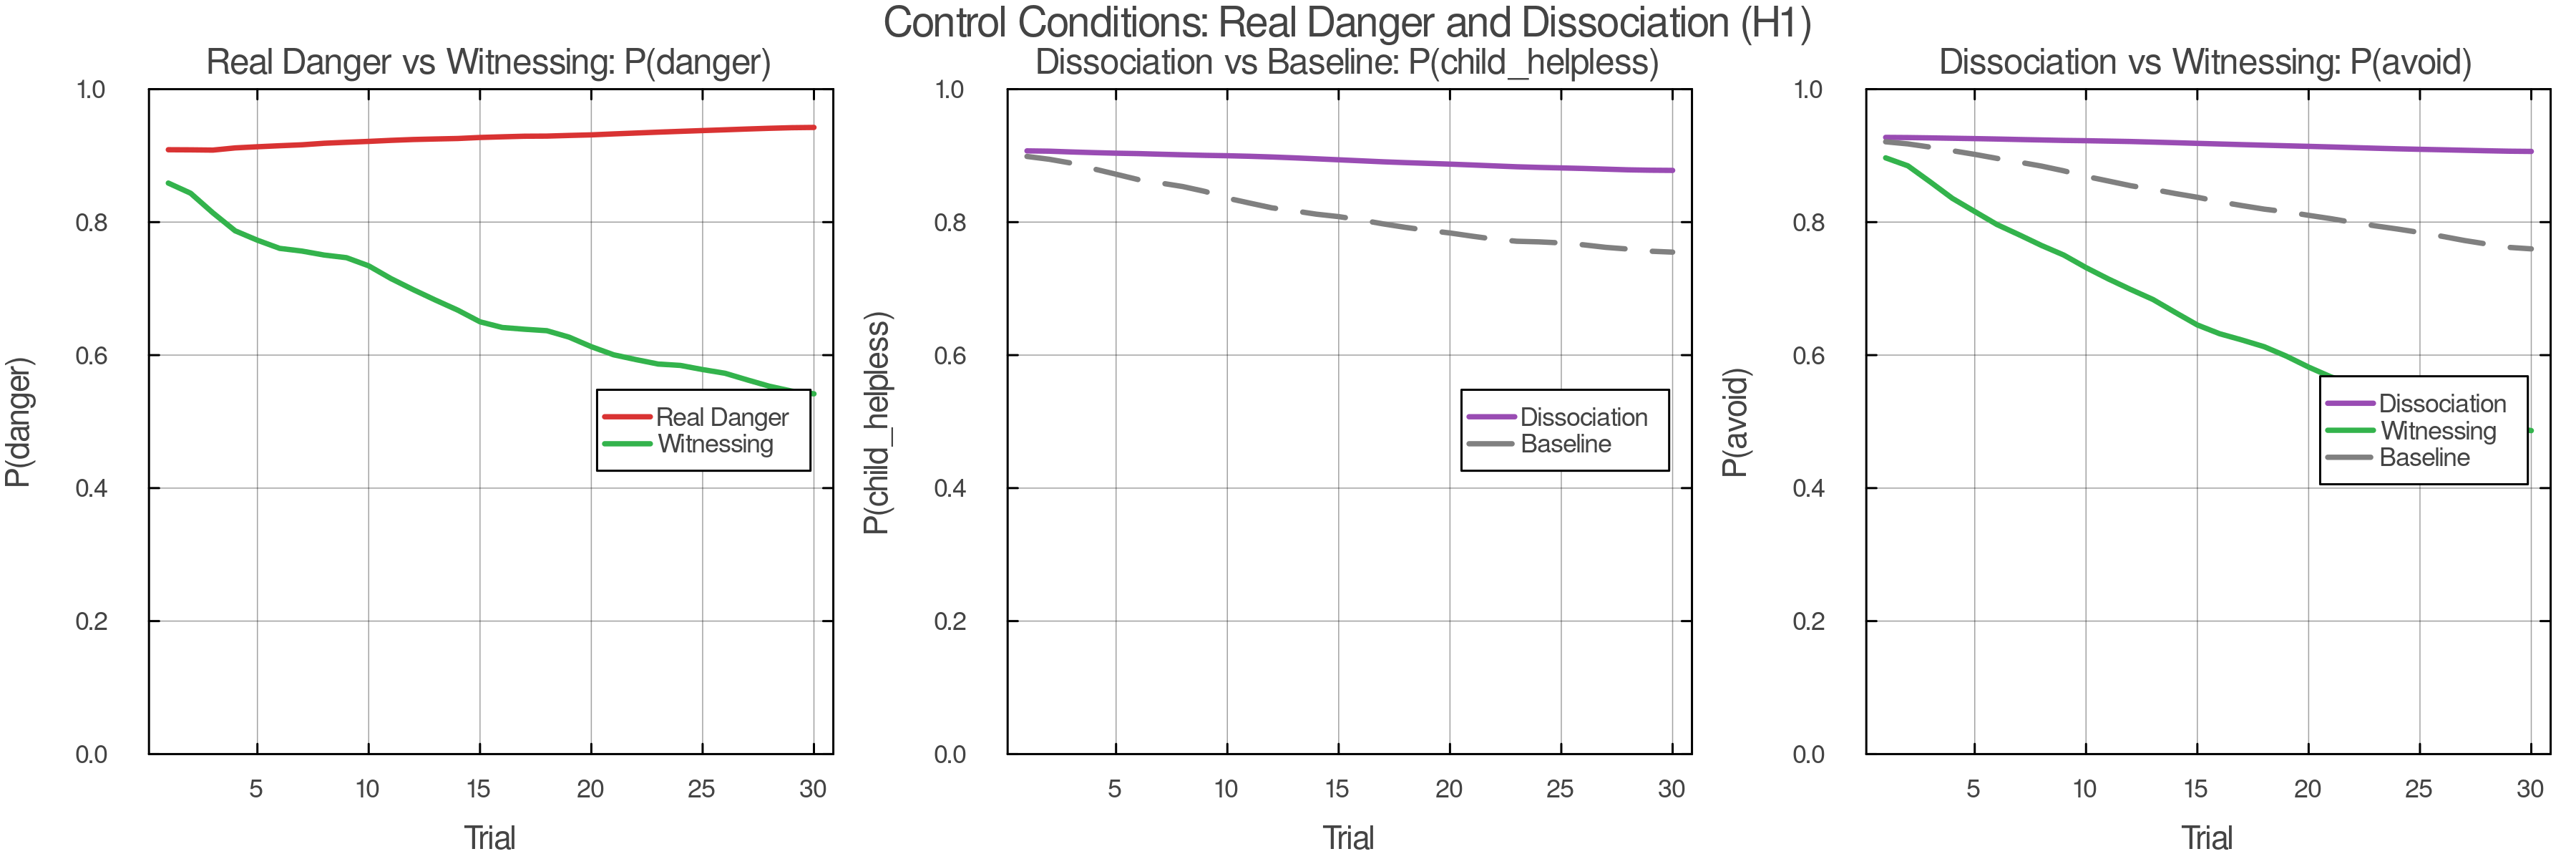
\includegraphics[keepaspectratio,alt={Figure: Control conditions showing dissociation vs witnessing profiles}]{figures/fig4_control_conditions.png}}
\caption{Figure: Control conditions showing dissociation vs witnessing
profiles}
\end{figure}

\emph{Figure 2. Control conditions. The real danger condition preserves
adaptive fear under high Self-energy. The dissociation condition reduces
disturbance without revising upstream priors --- distinguishing it from
genuine witnessing. The key discriminator is whether present-context
evidence remains online.}

\subsection{The 8 C's and self-like
parts}\label{the-8-cs-and-self-like-parts}

The 8 C's of Self --- calm, curiosity, clarity, compassion, confidence,
courage, creativity, connectedness --- can be read here as the
phenomenological signature of uncaptured inference under sufficiently
high Self-energy. That interpretation is respectful and minimal. It
honors the clinical observation without claiming to derive all eight
qualities from first principles.

The hardest test case is the self-like part: a manager that sounds
reflective, calm, and compassionate without actually producing the
inferential regime in which revision can occur. The model flags that
problem but does not solve it. A better account will have to separate
embodied regulation from reportable meta-awareness more sharply than a
single scalar allows.

\section{Blending and Witnessing}\label{blending-and-witnessing}

Same activation, different relationship. That is the paper's center of
gravity.

\subsection{Blending}\label{blending}

Blending occurs when an activated part captures inference. The part's
self-state, world-state, policy, and expected-outcome priors dominate
the posterior strongly enough that present context loses inferential
force. The person does not merely have fear. The fear organizes the
whole field.

Formally, blending corresponds to a high \textbf{capture index}:

\[
C_t = \frac{\pi^{\mathrm{eff}}_{\mathrm{part}}}{\pi^{\mathrm{eff}}_{\mathrm{part}} + \lambda^{\mathrm{eff}}_{\mathrm{ctx}}}
\]

where

\[
\pi^{\mathrm{eff}}_{\mathrm{part}} = r_t \cdot \pi_{\mathrm{part}} \cdot e^{-\beta E_t}
\]

and

\[
\lambda^{\mathrm{eff}}_{\mathrm{ctx}} = \lambda_{\mathrm{ctx}} \cdot e^{+\gamma E_t}
\]

Here $r_t$ is activation strength. Self-energy does not have to turn
activation off. It changes how much that activation can dominate.

Blending is graded, not binary. What varies is how much of the active
model becomes system-wide capture. Mild blending preserves some dual
awareness. Strong blending turns the part's beliefs into the only
available reality model.

\begin{figure}
\centering
\pandocbounded{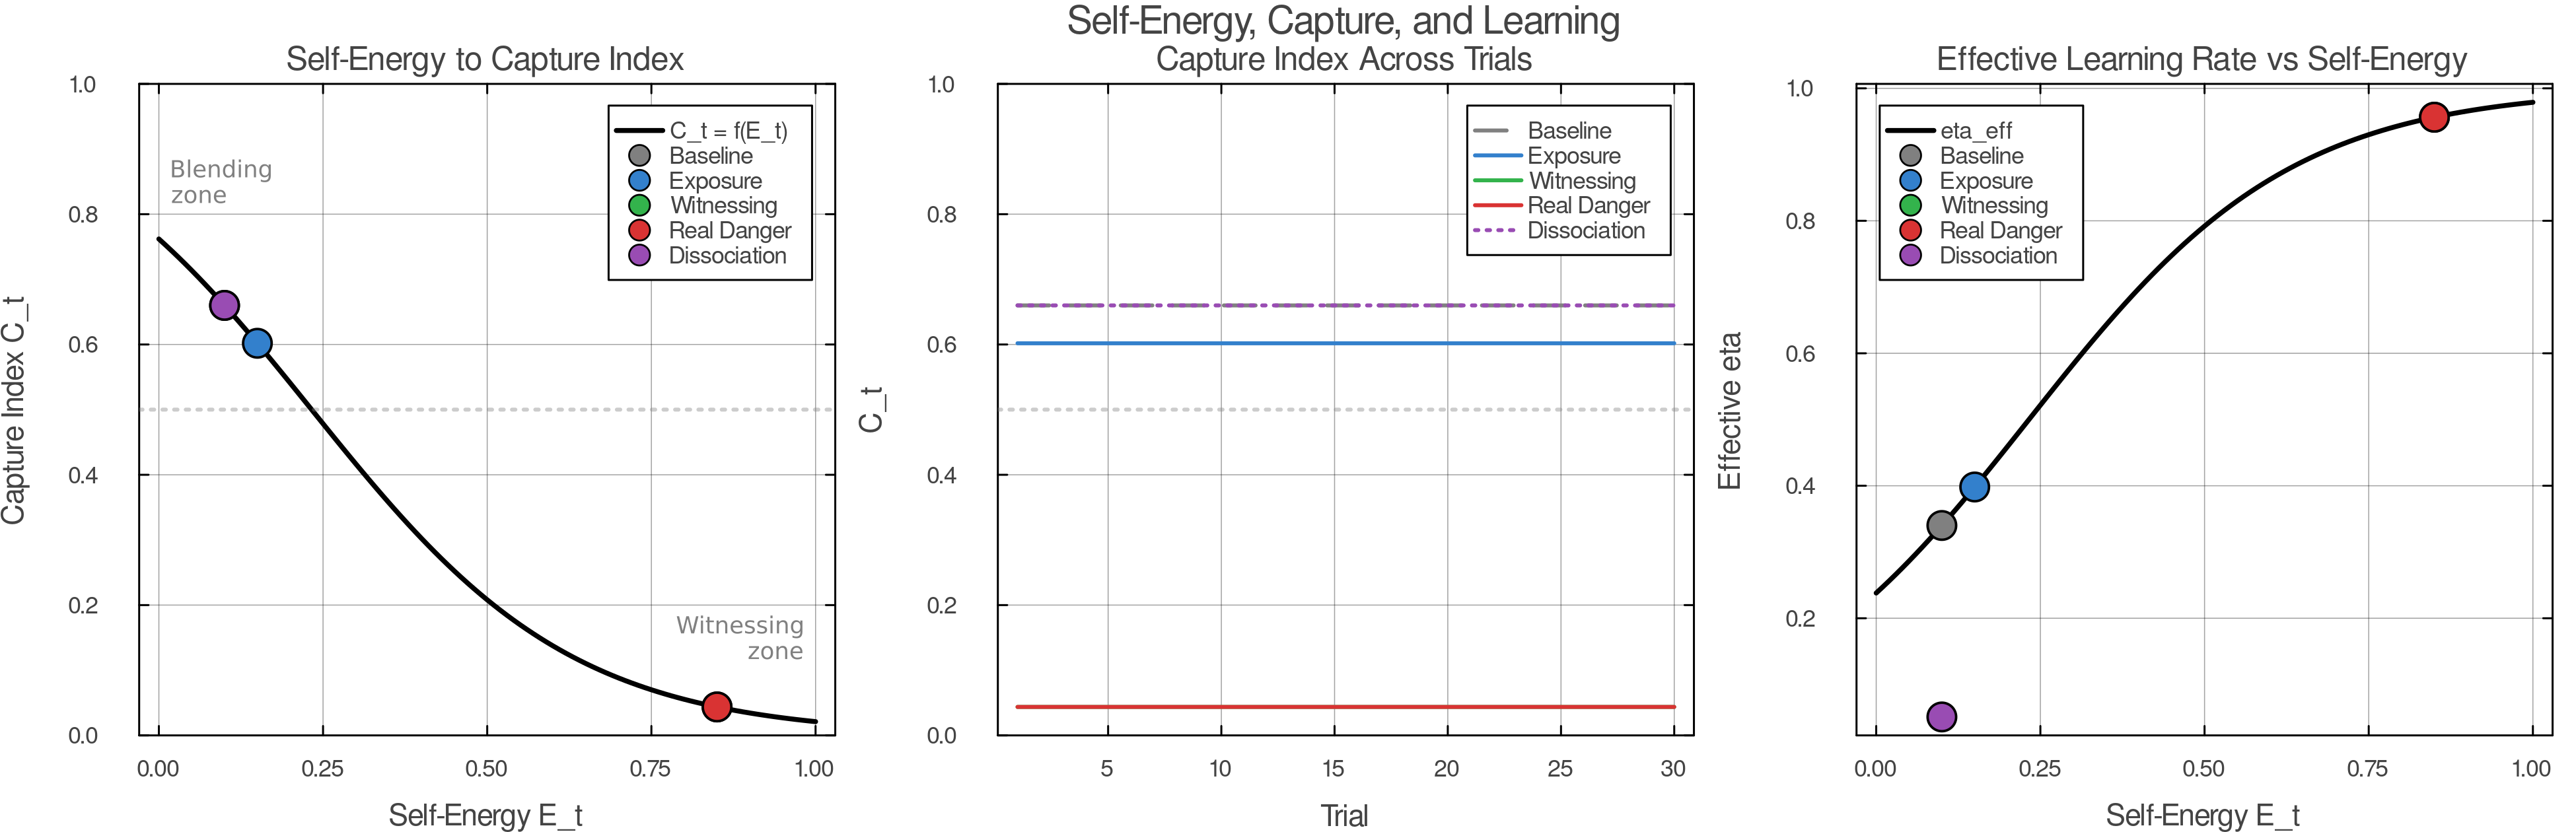
\includegraphics[keepaspectratio,alt={Figure: Capture index across conditions}]{figures/fig5_capture_index.png}}
\caption{Figure: Capture index across conditions}
\end{figure}

\emph{Figure 3. Capture index as a function of Self-energy. Low
Self-energy places baseline, exposure, and dissociation in the blending
zone. High Self-energy places witnessing in the context-held regime.
Capture is best read as a regime descriptor determined by the
condition-level Self-energy parameter.}

\subsection{Witnessing}\label{witnessing}

Witnessing is not the absence of activation. It is activation held in
context.

The part still fires. The body may still accelerate. The old priors
still come online. But present evidence stays online too: \emph{I am in
this room; I am with this therapist; this body is adult; this moment is
not the original one.} The activated part becomes something the system
can relate to rather than only speak from.

That is why witnessing is formally distinct from distraction,
suppression, or dissociation. Distraction lowers activation.
Dissociation lowers context impact. Witnessing leaves activation live
while preventing capture.

\subsection{The therapeutic zone}\label{the-therapeutic-zone}

The simplest way to picture the model is a 2x2 crossing part activation
and Self-energy.

{\def\LTcaptype{none} % do not increment counter
\begin{longtable}[]{@{}lll@{}}
\toprule\noalign{}
& Low Self-energy & High Self-energy \\
\midrule\noalign{}
\endhead
\bottomrule\noalign{}
\endlastfoot
\textbf{Low activation} & ordinary cognition & presence / Self \\
\textbf{High activation} & blending & witnessing \\
\end{longtable}
}

IFS therapy aims for the lower-right cell. That is difficult because the
cell is unstable by default. Activation tends to lower Self-energy. High
Self-energy tends to prevent full activation. Therapy therefore works by
titrating both at once: enough activation for the target priors to come
online, enough Self-energy for context to remain present.

\subsection{The clinical probe}\label{the-clinical-probe}

Clinicians do not ask for the capture index. They ask, ``How do you feel
toward this part?''

That question is a phenomenological assay of inferential regime. If the
client answers from the part --- \emph{I am terrified; I hate this; I
need to get away} --- the system is still captured by one bundle or
another. If the client answers with curiosity, compassion, calm
interest, or respectful distance, the system is more likely witnessing.
The question does not measure activation. It measures relationship to
activation. That is exactly what the model says matters.

\section{Why Only Witnessing Permits Lasting
Change}\label{why-only-witnessing-permits-lasting-change}

This section states the paper's main therapeutic claim.

Durable revision requires three conditions at once:

\begin{enumerate}
\def\labelenumi{\arabic{enumi}.}
\tightlist
\item
  \textbf{The part must be active.} Otherwise the target priors are
  dormant.
\item
  \textbf{Present context must be online.} Otherwise there is nothing to
  revise the priors with.
\item
  \textbf{The part must not capture inference.} Otherwise the mismatch
  between past model and present reality cannot register with enough
  force.
\end{enumerate}

Witnessing is the only regime that satisfies all three simultaneously.

\subsection{Why blending fails}\label{why-blending-fails}

Under blending, the part's priors dominate too strongly for present
contradiction to gain traction. The system may be surrounded by safety
and still infer danger because the active model interprets everything
through its own lens. The result is repetition without revision. The
part can activate thousands of times and remain essentially unchanged
because every activation happens inside the same local world.

\subsection{Why calm without activation
fails}\label{why-calm-without-activation-fails}

Calm by itself is not enough. A person can be regulated, insightful, and
articulate while the relevant bundle remains offline. In that case
nothing is live to revise. This is one reason understanding alone often
changes so little. Dormant priors do not update because they are not
currently generating predictions that can be contradicted.

\subsection{Unburdening as upstream
revision}\label{unburdening-as-upstream-revision}

At the algorithmic level, the paper interprets unburdening as durable
revision of upstream priors. In H1, self-state sits upstream of threat
meaning, which sits upstream of protective policy. A revision in
self-state --- from \emph{I am helpless here} to \emph{I am capable
here} --- changes what counts as dangerous. A change in threat meaning
changes what policies remain necessary.

This gives a formal answer to a familiar clinical observation: why does
deep change sometimes feel sudden? Because once an upstream prior shifts
far enough, several downstream expectations lose support together.

Clinically, unburdening often does more than reduce intensity. A part
that carried helplessness may, after unburdening, take on a new
functional role --- playfulness, healthy assertiveness, creativity. In
the present model, that transition corresponds to the bundle adopting
new policy priors and expected-outcome priors once the old self-state no
longer constrains the solution space. The formal account predicts
qualitative regime change, not merely damping.

\subsection{Exposure versus
witnessing}\label{exposure-versus-witnessing}

Exposure and witnessing both supply corrective contact under activation.
The difference is what variable they manipulate.

In this model, exposure forces contact while leaving Self-energy outside
the witnessing regime. Learning therefore occurs, but it occurs more
locally. Threat meaning can move. Specific stimulus-safety associations
can soften. Self-state can shift somewhat over time, but later, less
deeply, and with less generalization.

Witnessing changes the relation in which the same contact occurs. The
part remains live, but context now reaches the active priors more
directly. Under H1, that allows self-state revision to occur earlier and
to cascade forward.

The simulations support exactly that pattern. Under H1 witnessing,
self-state crosses the revision threshold first, threat meaning follows,
and avoidance lags. Under exposure, all three move more slowly and with
much less separation.

\begin{figure}
\centering
\pandocbounded{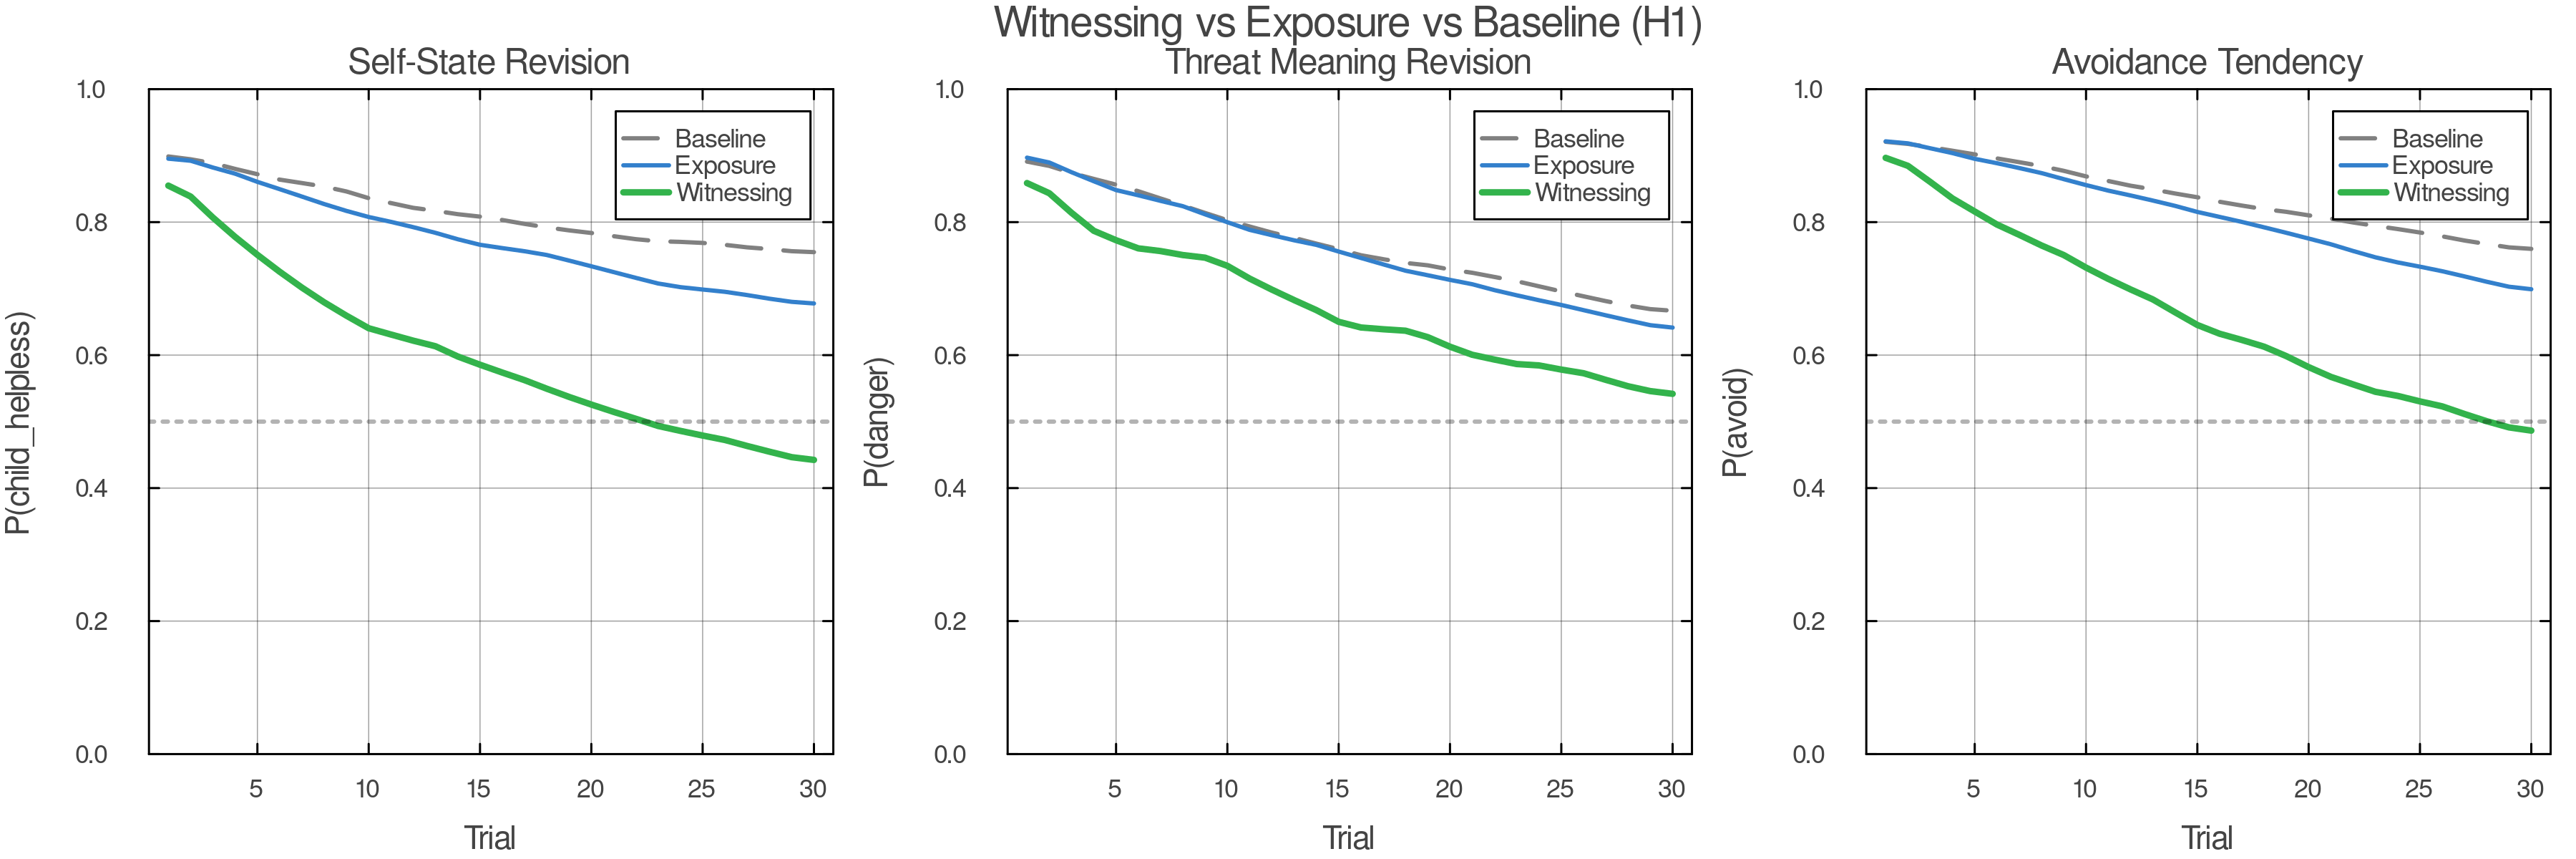
\includegraphics[keepaspectratio,alt={Figure: Witnessing vs exposure belief trajectories}]{figures/fig2_witnessing_vs_exposure.png}}
\caption{Figure: Witnessing vs exposure belief trajectories}
\end{figure}

\emph{Figure 4. Witnessing versus exposure under matched contact.
Witnessing produces faster and deeper revision across all three target
variables. The separation is attributable to inferential regime, not
privileged information --- the cue structure is identical across
conditions.}

\section{Protectors}\label{protectors}

Protectors are indispensable to clinical IFS. The model treats them
minimally, but not dismissively.

A protector is a learned policy prior plus an access-control tendency.
It prevents destabilizing takeover. That is already enough to explain
why protectors exist. If exile activation has historically led to
flooding, collapse, or unbearable pain, then preemptive management is
locally rational.

This is the core protector computation in the current model:

\begin{itemize}
\tightlist
\item
  if cue patterns predict that an exile may activate
\item
  and if available Self-energy is judged insufficient
\item
  then favor policies that reduce activation or block access to the
  exile
\end{itemize}

That minimal story already captures a great deal: avoidance,
intellectualization, perfectionism, numbing, distraction, rage, and
dissociation can all function as ways of preventing the wrong kind of
contact.

IFS distinguishes \textbf{managers} and \textbf{firefighters}. The
distinction maps cleanly onto temporal depth. Managers act
prospectively. They organize life to avoid entering dangerous
state-space in the first place. Firefighters act reactively. They
minimize acute free energy once danger has already broken through.

What the model does not yet formalize is equally important. Protectors
do not merely block. They negotiate. They assess trust. They have
conditions under which they will step back. A protector's willingness to
relax is not simply a function of reduced threat. It depends on whether
the protector believes Self is present enough, the context is safe
enough, and the process can be trusted. Computationally, that looks less
like a simple policy prior and more like a gate on information flow with
a learned trust variable. Those dynamics are clinically central and
formally deferred here.

\section{Multi-Part Polarization}\label{multi-part-polarization}

Single-part dynamics are not enough to describe actual inner life. One
of the most recognizable IFS phenomena is polarization: mutually
incompatible parts treating one another's preferred policies as
dangerous.

The mechanism is simple. Two bundles are active. Each assigns high cost
to the other's preferred action.

\begin{itemize}
\tightlist
\item
  Part A: \emph{approach, disclose, attach}
\item
  Part B: \emph{withdraw, protect, avoid}
\end{itemize}

Part A experiences withdrawal as abandonment and deadness. Part B
experiences approach as exposure and danger. Each therefore escalates in
response to the other. This is not merely conflict between
simultaneously represented preferences. It is often alternation between
rival local realities --- each side wholly true when it has the floor,
and each experiencing the other's preferred policy as threat.

Under low Self-energy, this produces the familiar phenomenology:
ambivalence, reversals, exhaustion, and the feeling that each side is
wholly true when it has the floor. Under high Self-energy, both remain
simultaneously representable without either taking over. A mixed or
negotiated policy becomes possible.

The polarization simulations support this reading. Under low
Self-energy, the two activations enter strong anti-phase oscillation.
Under high Self-energy, both remain simultaneously representable without
either taking over. A mixed or negotiated policy becomes possible.

One nuance is worth stating clearly. The summary metrics show that
\textbf{medium} Self-energy produces the highest policy entropy and
switching, while \textbf{high} Self-energy produces the most stable
simultaneous representation. That is not a bug. It suggests a transition
band. As capture weakens, the system first explores more combinations
and switches more often; once both parts can remain stably represented
together, switching drops and coexistence rises. That is clinically
plausible and theoretically useful.

\begin{figure}
\centering
\pandocbounded{\includegraphics[keepaspectratio,alt={Figure: Polarization dynamics across Self-energy levels}]{figures/polarization_combined.png}}
\caption{Figure: Polarization dynamics across Self-energy levels}
\end{figure}

\emph{Figure 5. Polarization dynamics. Low Self-energy produces
anti-phase oscillation between rival bundles. Medium Self-energy
increases exploration and switching. High Self-energy produces stable
simultaneous representation and reduced switching --- the transition
from capture to coexistence.}

\section{Simulation Design}\label{simulation-design}

The simulations are designed to test the paper's central claim in the
leanest case: same part, same cue channels, same architecture, different
inferential regime.

\subsection{Main model}\label{main-model}

The main simulation compares five conditions:

\begin{enumerate}
\def\labelenumi{\arabic{enumi}.}
\tightlist
\item
  \textbf{Baseline} --- safe world, low Self-energy, free policy
  selection
\item
  \textbf{Exposure} --- same safe world and cue structure, forced
  contact, Self-energy not elevated into the witnessing regime
\item
  \textbf{Witnessing} --- same contact as exposure, but with Self-energy
  elevated
\item
  \textbf{Real danger control} --- dangerous world under high
  Self-energy
\item
  \textbf{Dissociation control} --- safe world, low Self-energy, context
  impact reduced rather than genuinely maintained
\end{enumerate}

The part bundle begins with strong priors on child-helpless self-state,
danger meaning, and avoidance policy. The key comparison matches contact
across exposure and witnessing so that differences in updating are
attributable to inferential regime rather than privileged information.

\subsection{H1 versus H2}\label{h1-versus-h2}

The simulation compares two causal architectures.

\begin{itemize}
\tightlist
\item
  \textbf{H1: self-state upstream.} Present-context support informs
  self-state strongly; self-state conditions threat meaning; threat
  meaning conditions policy.
\item
  \textbf{H2: threat-primary.} Threat meaning is revised first;
  self-state follows.
\end{itemize}

This is not an arbitrary graph choice. H1 is motivated by the clinical
observation that parts often activate first as \emph{who I am here} ---
\emph{I am six; I am small; I am powerless} --- and that deep
therapeutic change is frequently experienced as a change in
identity-position before the world itself fully changes meaning. H2
remains a live competitor because many fear-learning models are
threat-primary. The point of the comparison is precisely to test which
ordering better fits the simulated dynamics.

\subsection{Formation and polarization
appendices}\label{formation-and-polarization-appendices}

Appendix A simulates part formation under three acquisition
environments: high threat plus low control, high threat plus high
control, and chronic low support. Appendix B simulates polarization
between two mutually threatening bundles under varying levels of
Self-energy.

\section{Results}\label{results}

The simulations support the core architecture of the paper.

\subsection{Same activation, different
relationship}\label{same-activation-different-relationship}

The first result is the simplest and the most important. Under matched
cue exposure, raising Self-energy changes the regime in which activation
occurs. Witnessing is not lower activation by another name. It is the
same activation held in a different relation.

In the H1 main simulation, the witnessing condition shows markedly
faster and deeper revision than exposure or baseline across all three
target variables. By the end of the run, witnessing reduces helpless
self-state, danger meaning, and avoidance far more than exposure does,
while baseline remains comparatively rigid. The separation is clear and
consistent with the theory.

\begin{figure}
\centering
\pandocbounded{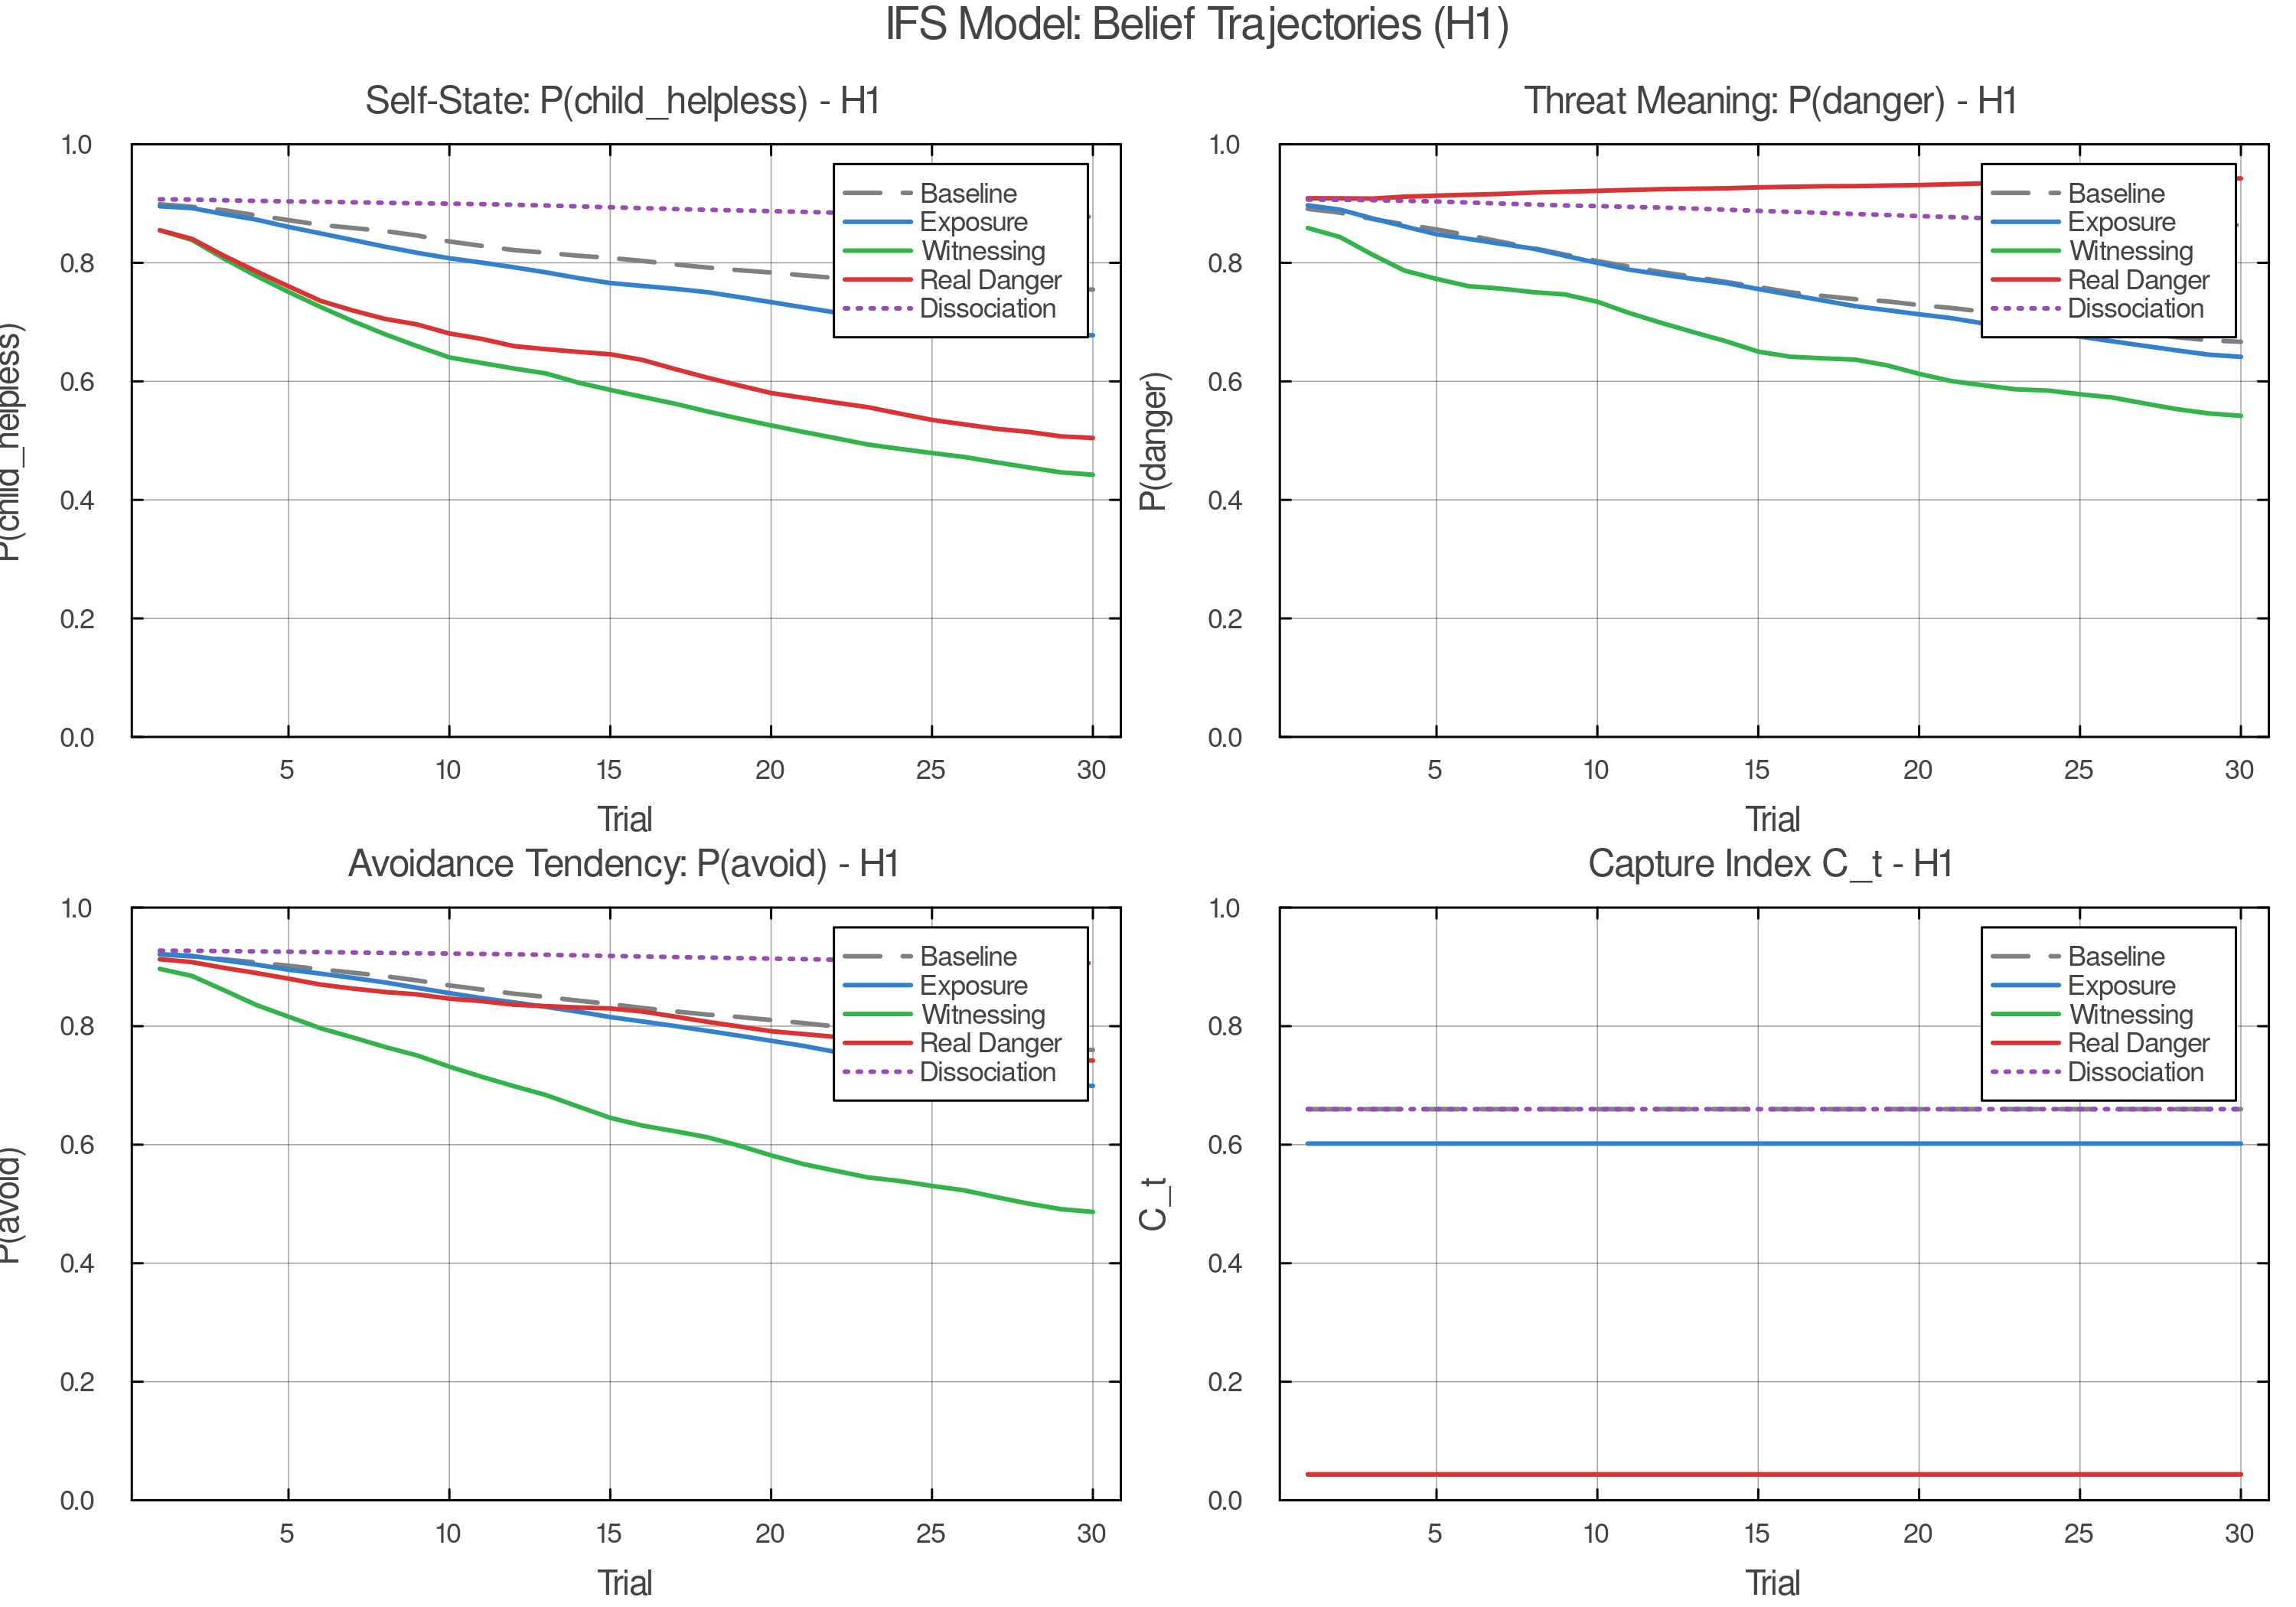
\includegraphics[keepaspectratio,alt={Figure: H1 belief trajectories across conditions}]{figures/fig1_h1_belief_trajectories.png}}
\caption{Figure: H1 belief trajectories across conditions}
\end{figure}

\emph{Figure 6. H1 belief trajectories. Witnessing (green) produces the
deepest revision across self-state, threat meaning, and avoidance.
Exposure (blue) learns but more slowly and uniformly. Baseline (grey)
shows minimal movement. The separation is attributable to inferential
regime under matched contact.}

\subsection{H1 produces the predicted revision
order}\label{h1-produces-the-predicted-revision-order}

Under H1 witnessing, self-state revises first. The child-helpless prior
crosses the chosen threshold at trial 9. Threat meaning follows at trial
13. Avoidance declines last and only later approaches the same
threshold. This is the exact ordering the model predicts if self-state
is upstream of threat meaning and threat meaning is upstream of policy.

The exposure condition does not show that ordering clearly. All three
trajectories move together more slowly. The system learns, but it learns
locally and without the same cascade.

\begin{figure}
\centering
\pandocbounded{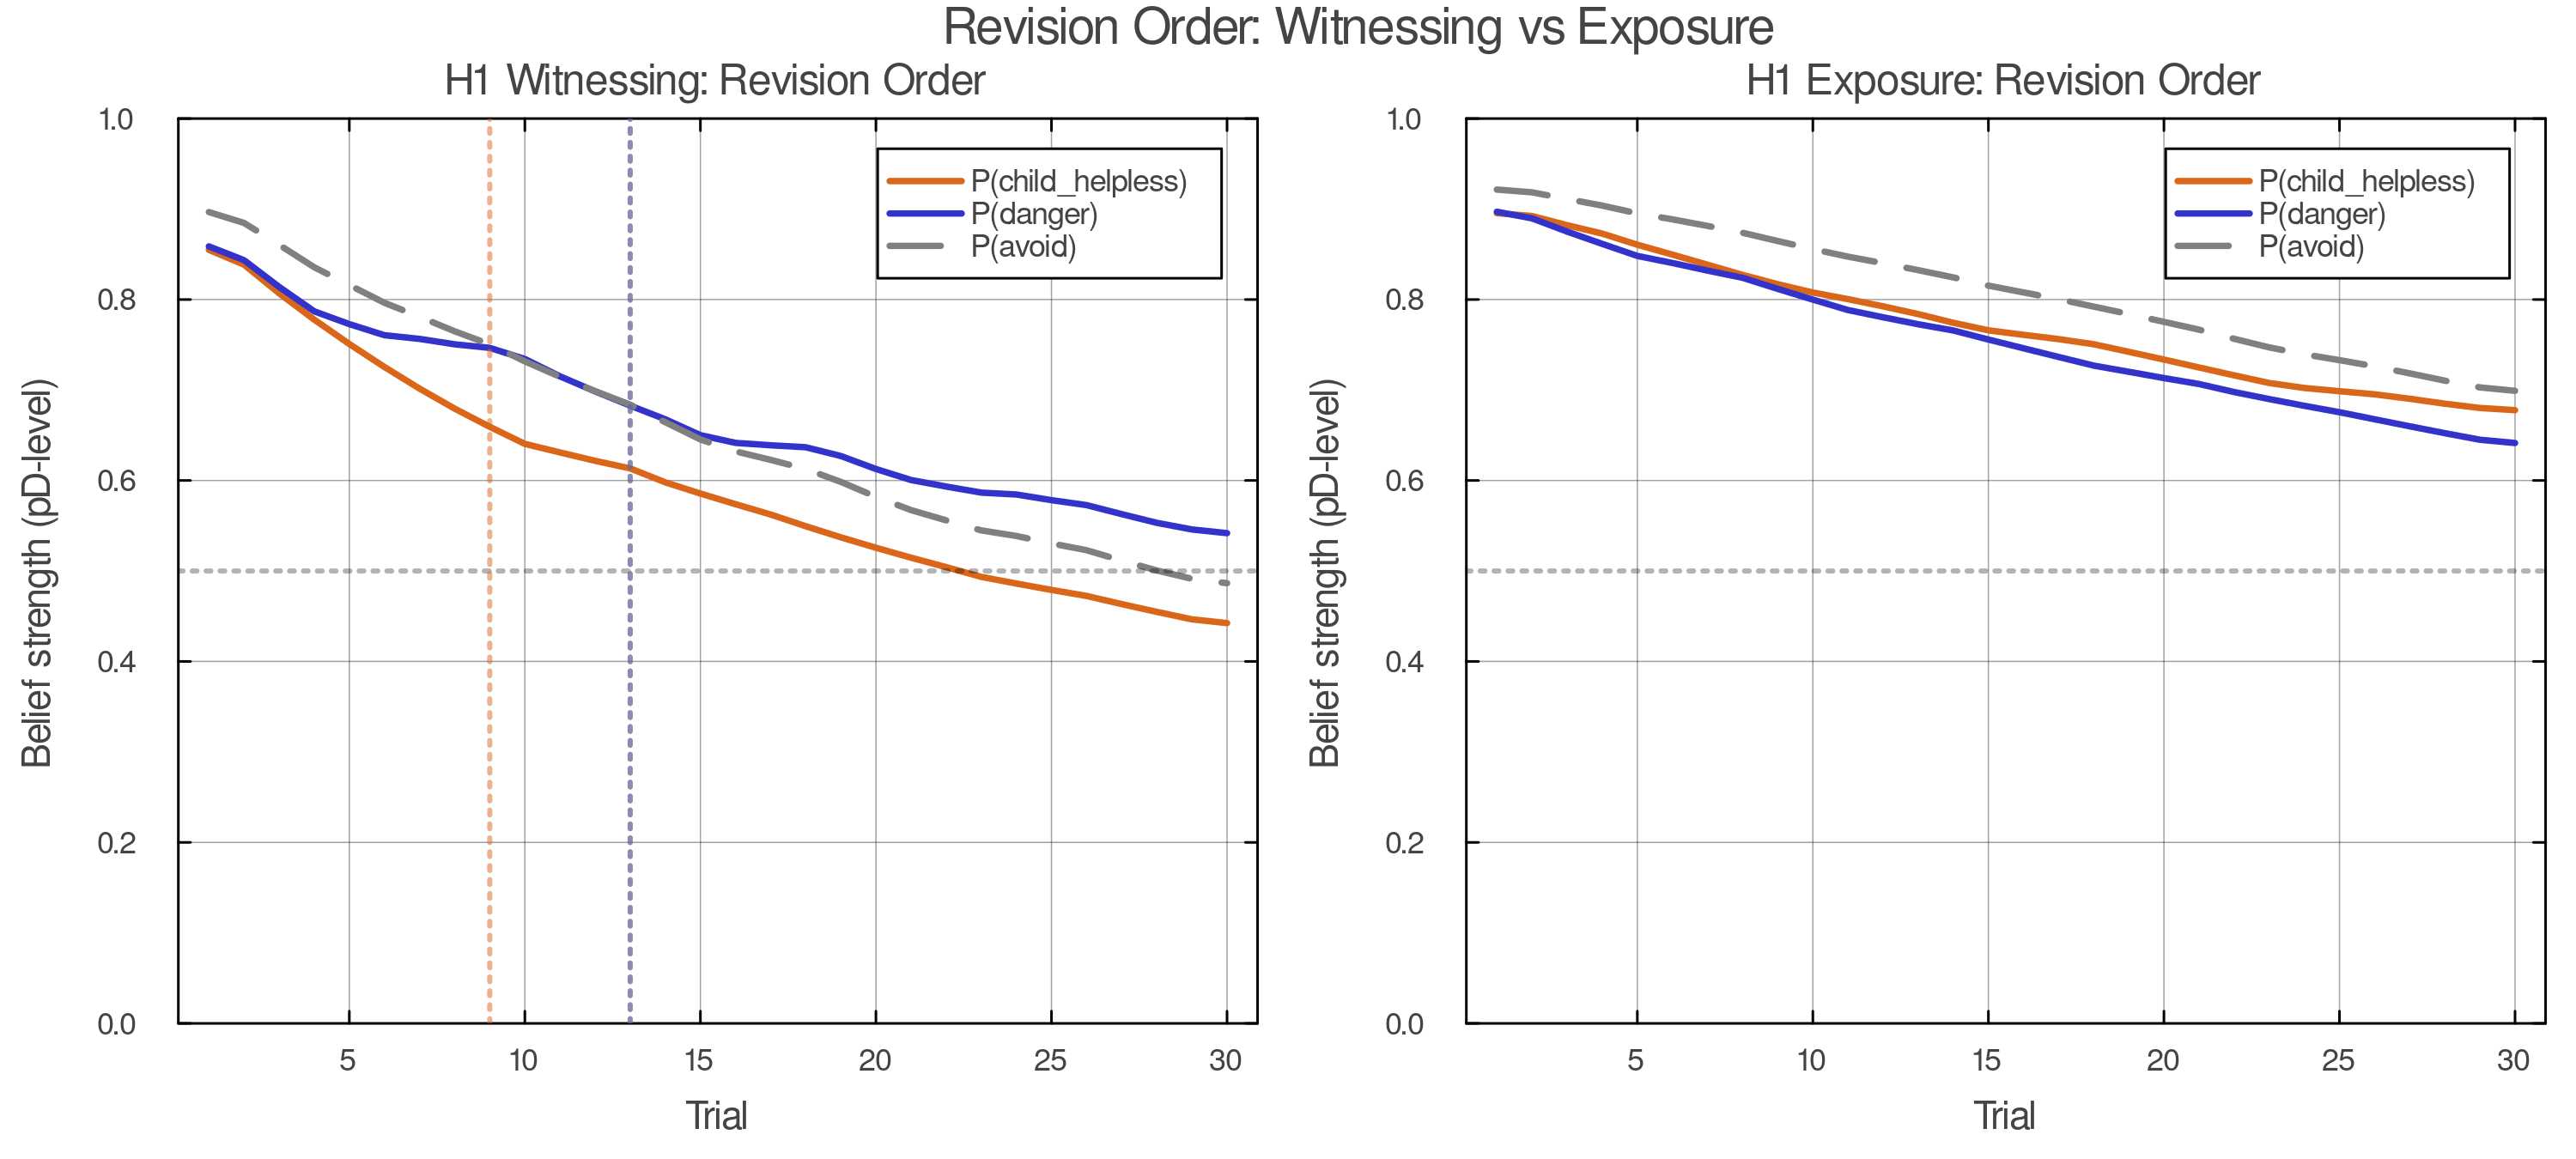
\includegraphics[keepaspectratio,alt={Figure: Revision order under H1 vs H2}]{figures/fig6_revision_order.png}}
\caption{Figure: Revision order under H1 vs H2}
\end{figure}

\emph{Figure 7. Revision order comparison. H1 witnessing produces the
predicted cascade: self-state first, threat meaning second, avoidance
last. H2 reverses the order, with threat meaning leading. The ordering
difference is the paper's main model comparison.}

\subsection{H2 flips the order}\label{h2-flips-the-order}

The H1/H2 comparison comes out in the right place. Under H2, danger
meaning moves earlier and self-state lags. That is the opposite of the
IFS-consistent prediction. The bar summary of threshold crossings makes
the contrast legible: H1 gives \textbf{child first, danger second}; H2
gives \textbf{danger first, child later}. This is the paper's main model
comparison.

\begin{figure}
\centering
\pandocbounded{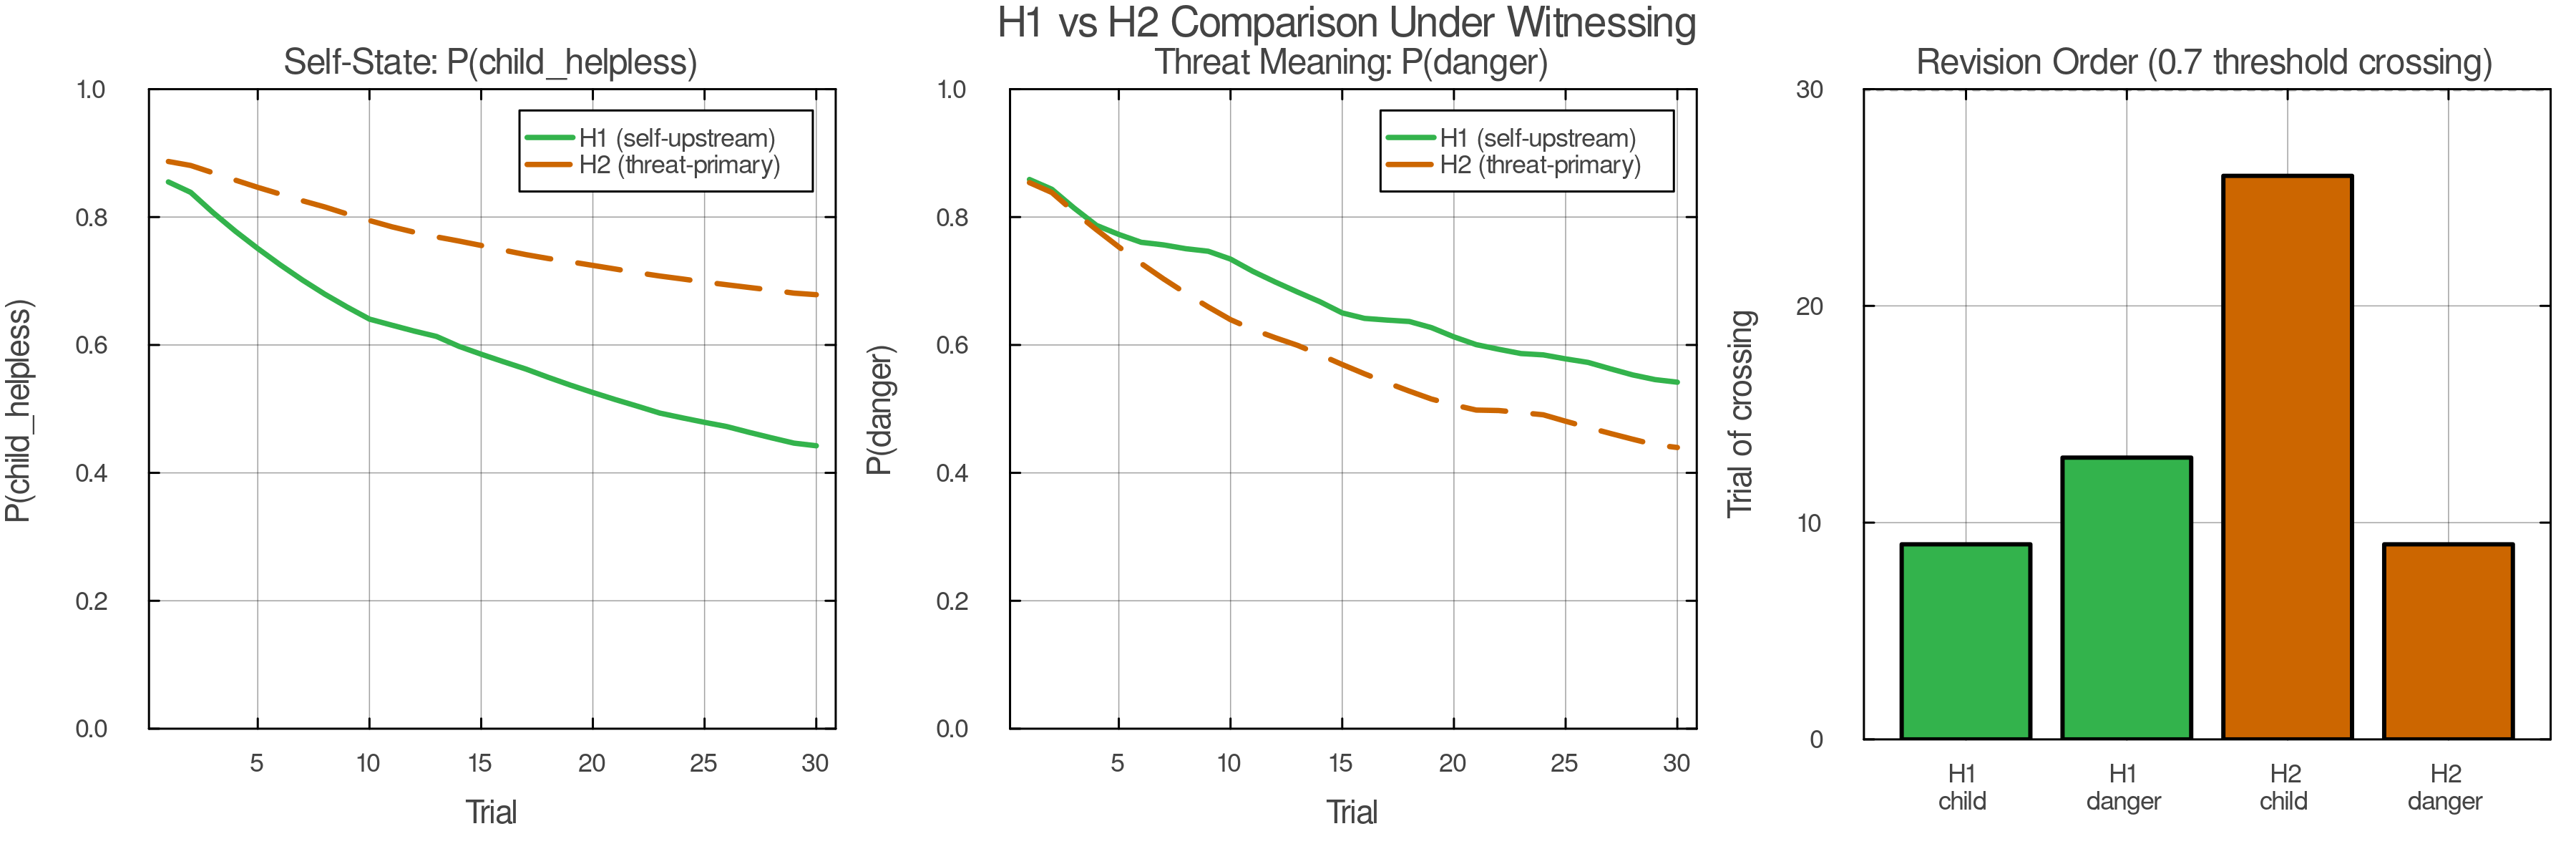
\includegraphics[keepaspectratio,alt={Figure: H1 vs H2 witnessing trajectories}]{figures/fig3_h1_vs_h2_witnessing.png}}
\caption{Figure: H1 vs H2 witnessing trajectories}
\end{figure}

\emph{Figure 8. H1 versus H2 under witnessing. The two architectures
produce different revision cascades. H1 revises self-state upstream,
consistent with IFS clinical observation. H2 revises threat meaning
first, consistent with threat-primary fear-learning models.}

\subsection{Witnessing outperforms exposure without changing the
task}\label{witnessing-outperforms-exposure-without-changing-the-task}

The witnessing versus exposure comparison is one of the paper's
strongest results because the task is matched. The system sees the same
kinds of cues and undergoes the same kind of contact. The difference is
inferential regime, not information. Witnessing therefore does not win
by being handed a privileged channel. It wins because Self-energy
changes the precision balance between the active bundle and present
context.

\subsection{Real danger preserves adaptive
fear}\label{real-danger-preserves-adaptive-fear}

The real danger control does exactly what it needs to do. Under genuine
danger, the model does not collapse into indiscriminate calm. Threat
meaning remains high even under high Self-energy. This is a sanity check
and a theoretical constraint. Self-energy does not abolish fear. It
preserves the possibility of accurate fear.

One nuance deserves explicit interpretation. In the real-danger
condition, threat meaning remains high while helpless self-state still
softens relative to its initial value. This is not incoherent. The
system can learn \emph{this is dangerous} without also learning
\emph{therefore I am a child and helpless}. That distinction is
clinically welcome. Mature fear does not require regressive identity.

\subsection{Dissociation is not
witnessing}\label{dissociation-is-not-witnessing}

The dissociation control is equally important. It reduces disturbance
without producing the same revision profile as witnessing. Self-state
barely moves. Avoidance remains high. The system is quieter, but the old
priors remain largely intact.

That is exactly the distinction the paper needs. Calm is not enough.
What matters is whether context stays online or is functionally turned
down.

\subsection{Capture is a regime parameter in the current
simulations}\label{capture-is-a-regime-parameter-in-the-current-simulations}

The capture index figure shows the mapping from Self-energy to capture
clearly. Low Self-energy places baseline, exposure, and dissociation in
the blending zone; high Self-energy places witnessing in the
context-held regime. In the current implementation, capture is set by
the condition-level Self-energy parameter, which is why it remains
constant across trials within a given condition. In this implementation,
capture is best read as a \textbf{regime descriptor} rather than a
learning-dependent time series.

\subsection{Formation depends strongly on low
control}\label{formation-depends-strongly-on-low-control}

The formation appendix supports the threat-plus-low-control claim. High
threat with low control produces the strongest final bundle rigidity.
Chronic low support produces an intermediate profile. High threat with
high control produces substantially weaker helpless self-state
consolidation.

\textbf{Control chiefly gates whether threat learning hardens into
identity-level bundle rigidity.} Threat meaning and avoidance rise
across conditions, but low control most strongly sharpens the helpless
self-state and the integrated bundle measure. High-control threat still
produces learning, but much less identity-level consolidation.

\subsection{Polarization is mutual threat plus
capture}\label{polarization-is-mutual-threat-plus-capture}

The polarization appendix also behaves well. Low Self-energy produces
the expected oscillatory alternation between the two bundles. High
Self-energy produces prolonged simultaneous representation and sharp
reductions in policy switching. Medium Self-energy increases entropy and
switching before the system settles into stable coexistence. Read
clinically, the model suggests a transition from capture, to
exploration, to negotiation.

\begin{figure}
\centering
\pandocbounded{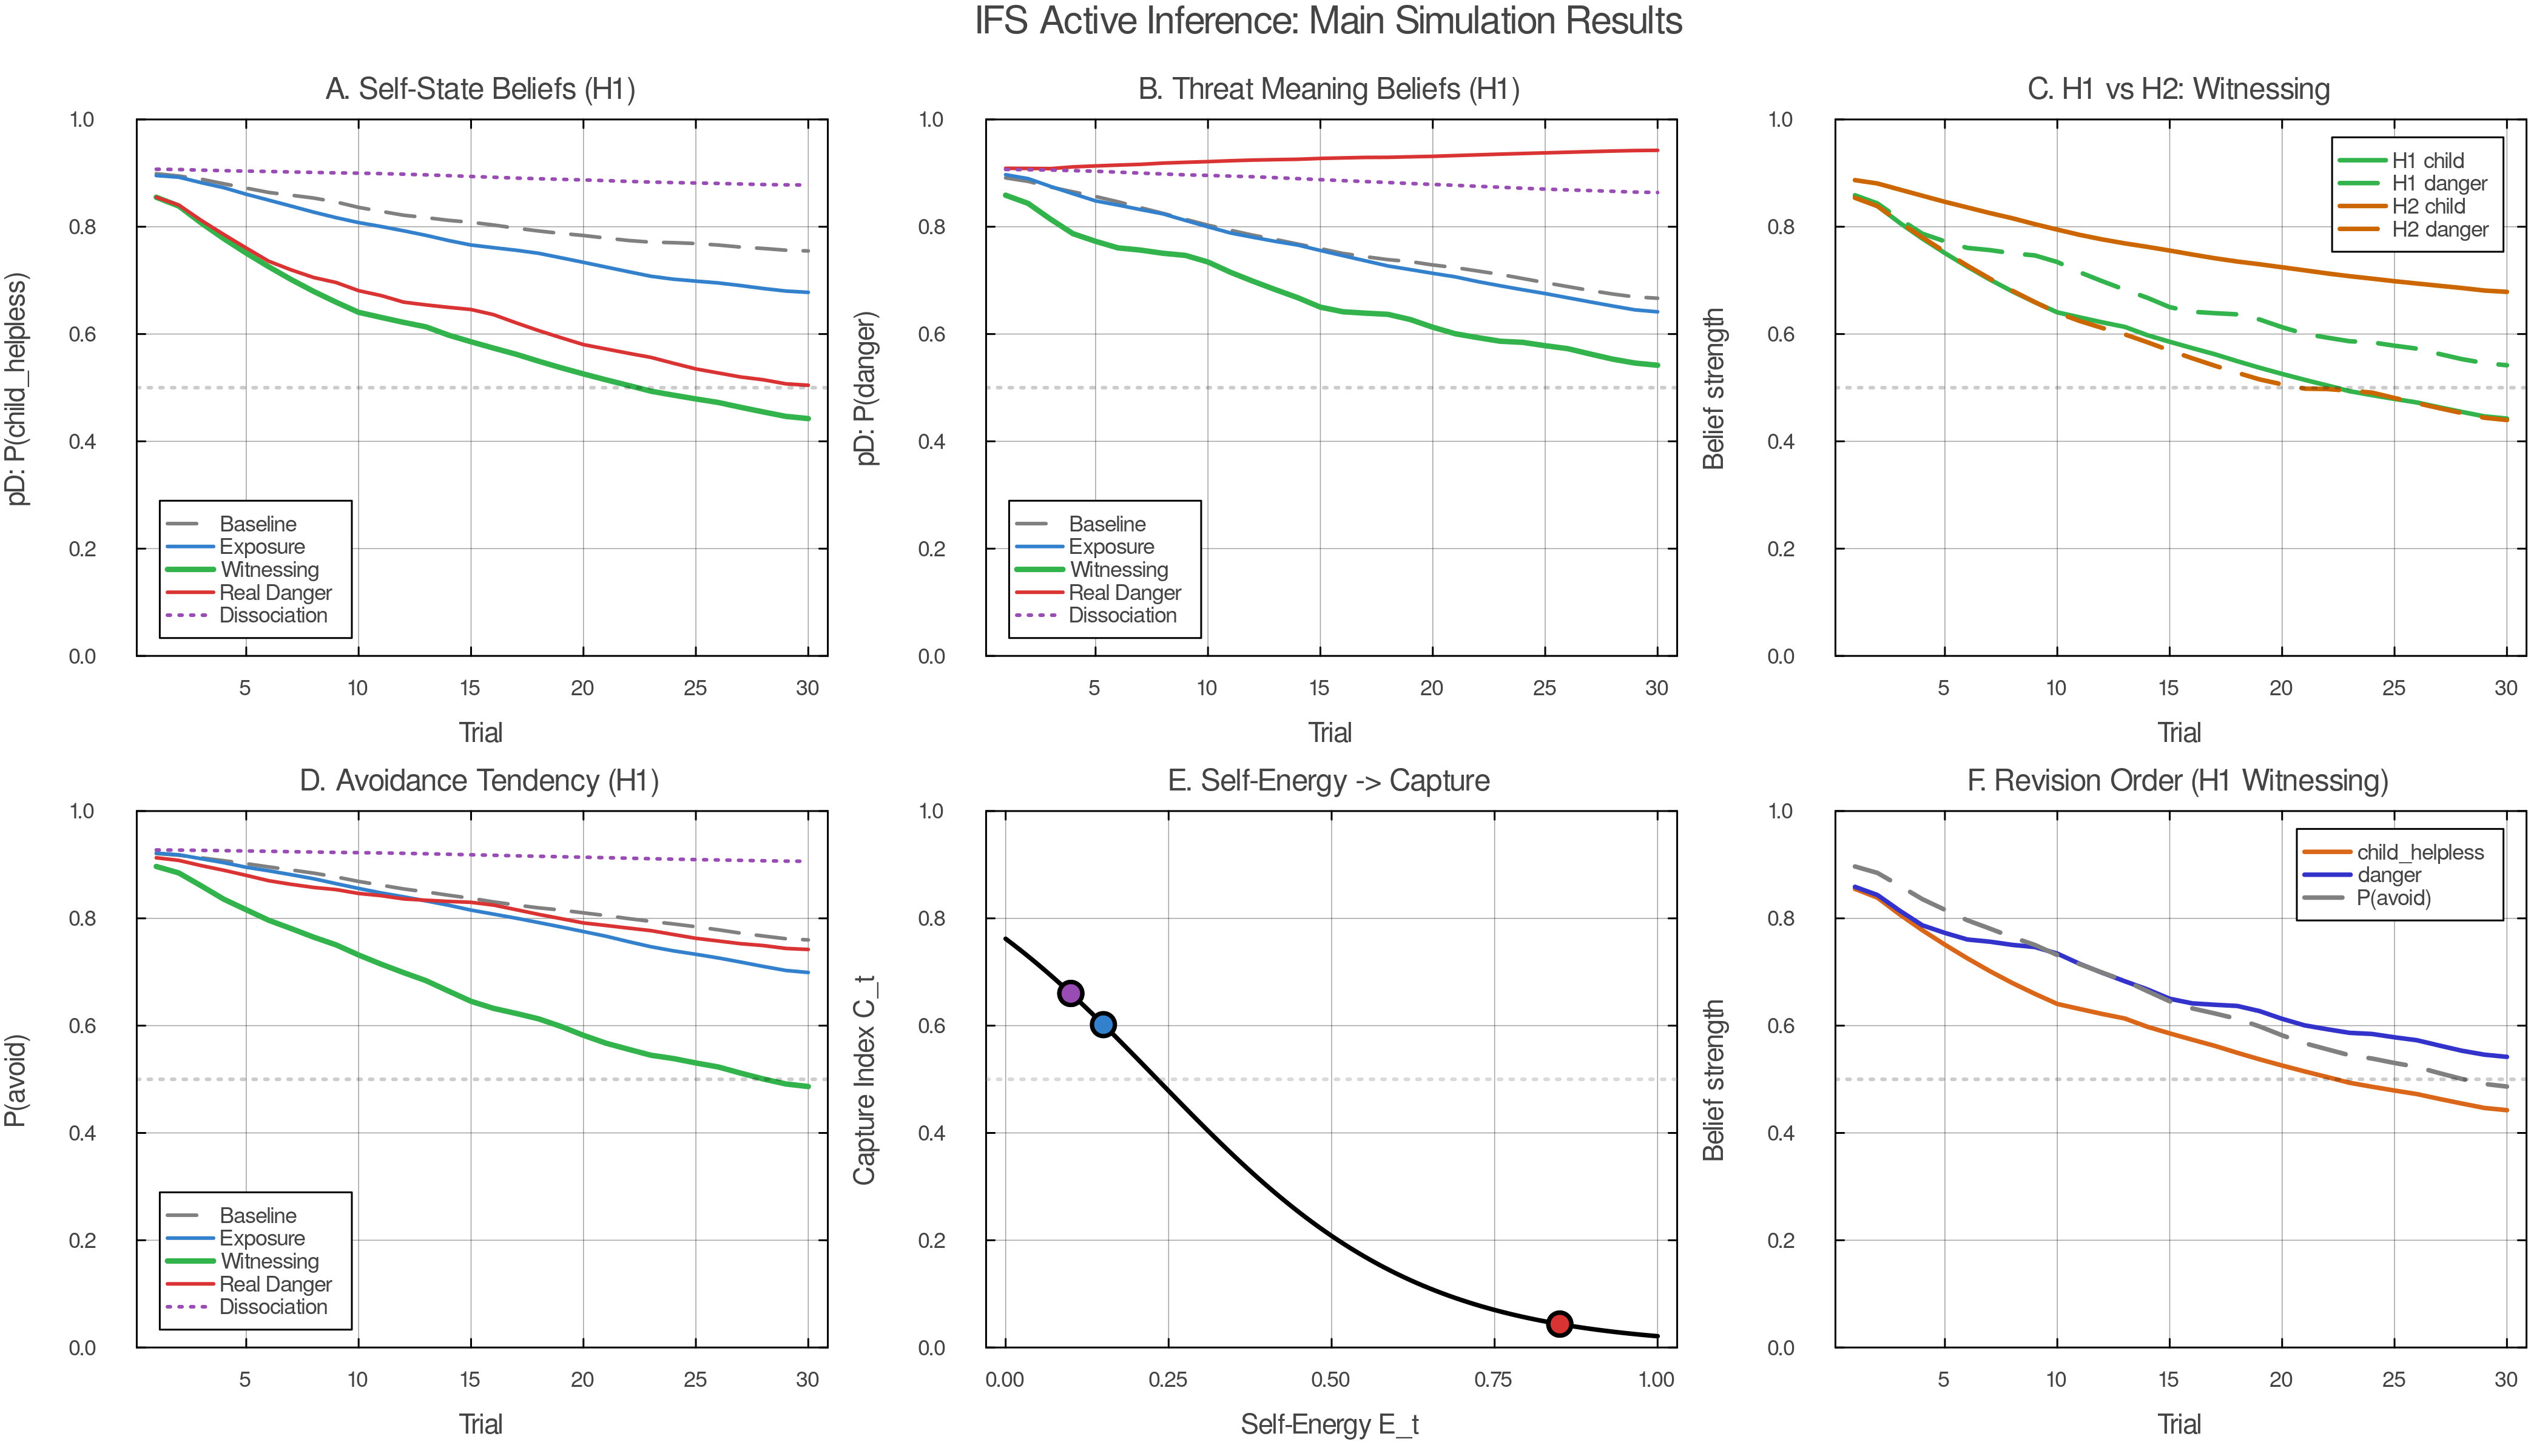
\includegraphics[keepaspectratio,alt={Figure: Main simulation summary}]{figures/fig7_main_summary.png}}
\caption{Figure: Main simulation summary}
\end{figure}

\emph{Figure 9. Main simulation summary. Final belief states across all
five conditions for self-state, threat meaning, and avoidance.
Witnessing produces the deepest revision. Exposure produces intermediate
revision. Baseline and dissociation leave priors largely intact. Real
danger preserves adaptive threat meaning.}

\section{Discussion}\label{discussion}

The paper set out to answer a narrow but clinically important question:
when a part activates, what determines whether it takes over or can be
held in context, and why does only the latter permit lasting change?

The answer proposed here is structural. Self-energy governs the
precision balance between active part priors and present-context
evidence. That balance determines inferential regime. Under blending,
the part captures the field. Under witnessing, the same part remains
active while context stays online. That difference is enough to explain
why some activations merely repeat a prior and others revise it.

\subsection{What the model explains}\label{what-the-model-explains}

The account explains five things without too much machinery.

First, it explains why parts feel like whole worlds rather than isolated
beliefs. The bundle structure couples self-state, world-state, policy,
and outcome.

Second, it explains why activation alone is not therapeutic. Without
context, activation repeats. Without activation, context cannot reach
the dormant prior. Witnessing uniquely provides both.

Third, it explains why IFS-like change often feels upstream and
generalizing. Under H1, revising self-state changes what counts as
dangerous, which then changes what protectors need to do.

Fourth, it distinguishes Self-led calm from dissociative quiet. Both may
look regulated. Only one preserves contact.

Fifth, it shows why this still counts as an IFS model despite being
minimal. What makes the model specifically IFS is not plurality alone.
It is the claim that the decisive therapeutic variable is the
Self-mediated relation to activated part-content.

\subsection{What it does not yet
explain}\label{what-it-does-not-yet-explain}

The paper also leaves several clinically important structures
under-modeled.

It does not yet formalize full protector negotiation. Protectors in
clinical IFS do not merely block --- they compute trust, grant
permission, and have conditions under which they will step back. The
current model captures the blocking function but not the relational
intelligence that makes IFS's protector work distinctive. It does not
distinguish genuine Self from self-like managerial imitation --- a
distinction that probably requires separating embodied regulation from
reportable meta-awareness more sharply than a single scalar allows. It
does not model the therapist as a second agent, even though the clinical
process is often dyadic long before it becomes stably intra-psychic. And
it does not yet scale from one activated bundle or one polarity pair to
a full inner parliament.

These are real absences. They are also the right absences for a first
model. The ambition here is not comprehensiveness. It is to get the core
mechanism right before expanding the frame.

\subsection{Implications for therapy
comparison}\label{implications-for-therapy-comparison}

The strongest comparative implication concerns exposure. The paper does
not claim that exposure fails. The simulations show the opposite:
exposure learns. What they show is that exposure and witnessing learn
differently.

Exposure alters threat expectations under contact. Witnessing alters the
relation in which that contact occurs. If self-state truly sits
upstream, then witnessing should revise a broader class of downstream
appraisals. That is the paper's clearest comparative claim and probably
its cleanest empirical target.

\subsection{Next steps}\label{next-steps}

The next extensions are now obvious.

\begin{enumerate}
\def\labelenumi{\arabic{enumi}.}
\tightlist
\item
  \textbf{Dyadic regulation:} model therapist and client as interacting
  agents rather than hiding co-regulation inside one scalar support
  term.
\item
  \textbf{Self-like parts:} separate autonomic regulation from
  meta-awareness and test which combinations produce revision versus
  pseudo-witnessing.
\item
  \textbf{Richer protector computation:} formalize trust, conditional
  permission, and role transformation.
\item
  \textbf{Multi-part networks:} move from one polarity pair to several
  coupled bundles with different developmental ages and policies.
\item
  \textbf{Empirical fitting:} align simulated trajectory measures with
  session-level data, especially revision order and generalization
  gradients.
\end{enumerate}

This paper does not finish the job. It builds the first floor. That is
enough, at least for now, if the floor holds.

\section{Appendix A. Formation
Simulation}\label{appendix-a.-formation-simulation}

\begin{figure}[H]
\centering
\includegraphics[width=0.92\linewidth]{formation_acquisition_trajectories.png}
\caption{Formation acquisition trajectories across the three development conditions.}
\label{fig:formation-acquisition-v5}
\end{figure}
\FloatBarrier

\begin{figure}[H]
\centering
\includegraphics[width=0.92\linewidth]{formation_controllability_gradient.png}
\caption{Controllability gradient in part formation. Low control is the main driver of helpless self-state consolidation and bundle rigidity.}
\label{fig:formation-control-v5}
\end{figure}
\FloatBarrier

\begin{figure}[H]
\centering
\includegraphics[width=0.92\linewidth]{formation_bundle_rigidity.png}
\caption{Bundle rigidity by acquisition environment. High threat plus low control produces the strongest integrated rigidity profile.}
\label{fig:formation-rigidity-v5}
\end{figure}
\FloatBarrier

\begin{figure}[H]
\centering
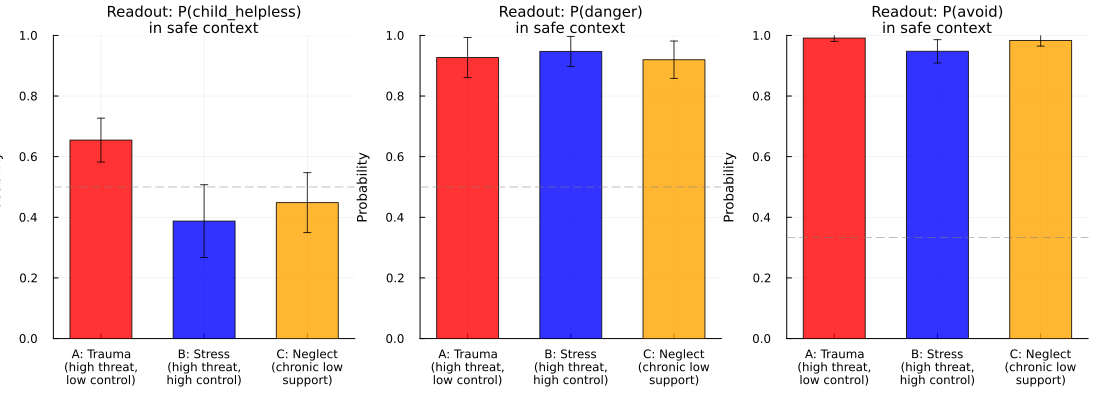
\includegraphics[width=0.92\linewidth]{formation_readout_comparison.png}
\caption{Safe-context readout after formation. The low-control condition carries the strongest residual bundle into safety.}
\label{fig:formation-readout-v5}
\end{figure}
\FloatBarrier

The formation simulation asks a simple question: can part-like bundle
rigidity arise through precision-weighted learning alone, without
assuming literal graph surgery?

The answer from the current simulation is yes, with one important
refinement. All three acquisition environments produce some learning,
but not the same kind of learning.

\begin{itemize}
\tightlist
\item
  \textbf{High threat + low control} produces the strongest helpless
  self-state consolidation and the highest integrated bundle rigidity.
\item
  \textbf{High threat + high control} produces strong danger learning
  but much weaker helpless self-state consolidation.
\item
  \textbf{Chronic low support} produces an intermediate, slower-forming
  profile.
\end{itemize}

This pattern supports the formation account. The critical ingredient is
not fear in isolation. It is fear under insufficient control or
co-regulation. The readout in a safe context makes that visible: the
low-control condition carries the strongest residual bundle into safety.

\textbf{Low control converts threat learning into identity-weighted part
formation.}

\begin{figure}
\centering
\pandocbounded{\includegraphics[keepaspectratio,alt={Figure: Formation acquisition trajectories}]{figures/formation_acquisition_trajectories.png}}
\caption{Figure: Formation acquisition trajectories}
\end{figure}

\emph{Figure A1. Acquisition trajectories across three formation
conditions. High threat with low control produces the strongest and
fastest consolidation of the full bundle (self-state, threat meaning,
avoidance).}

\begin{figure}
\centering
\pandocbounded{\includegraphics[keepaspectratio,alt={Figure: Formation controllability gradient}]{figures/formation_controllability_gradient.png}}
\caption{Figure: Formation controllability gradient}
\end{figure}

\emph{Figure A2. Controllability gradient. As perceived control
increases, helpless self-state consolidation weakens sharply while
threat learning persists --- supporting the claim that control gates
identity-level bundle formation.}

\section{Appendix B. Polarization
Simulation}\label{appendix-b.-polarization-simulation}

\begin{figure}[H]
\centering
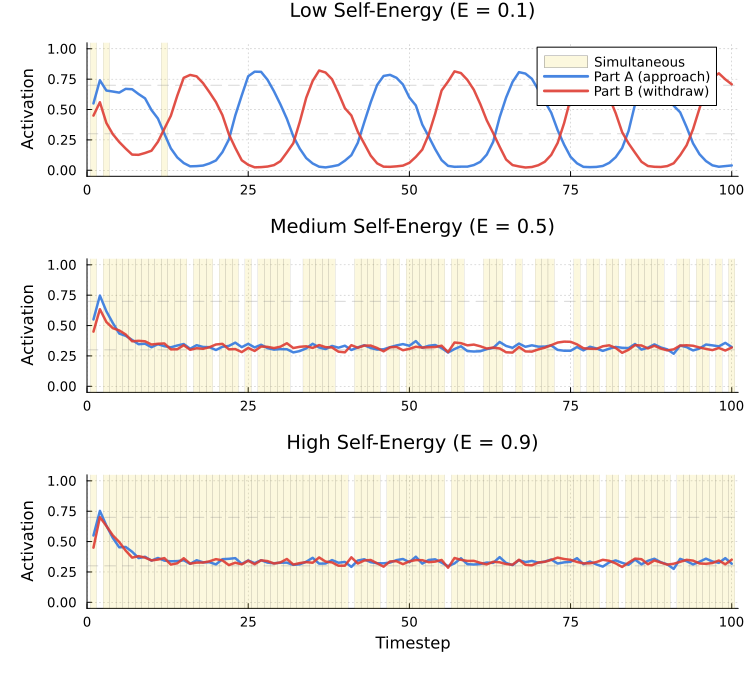
\includegraphics[width=0.92\linewidth]{polarization_timeseries.png}
\caption{Polarization time series. Low Self-energy produces strong anti-phase alternation between the two bundles.}
\label{fig:polarization-timeseries-v5}
\end{figure}
\FloatBarrier

\begin{figure}[H]
\centering
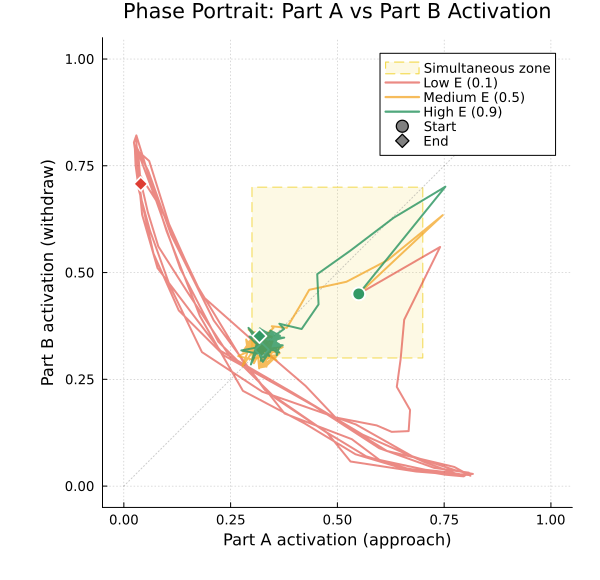
\includegraphics[width=0.92\linewidth]{polarization_phase.png}
\caption{Polarization phase portrait under varying Self-energy levels.}
\label{fig:polarization-phase-v5}
\end{figure}
\FloatBarrier

\begin{figure}[H]
\centering
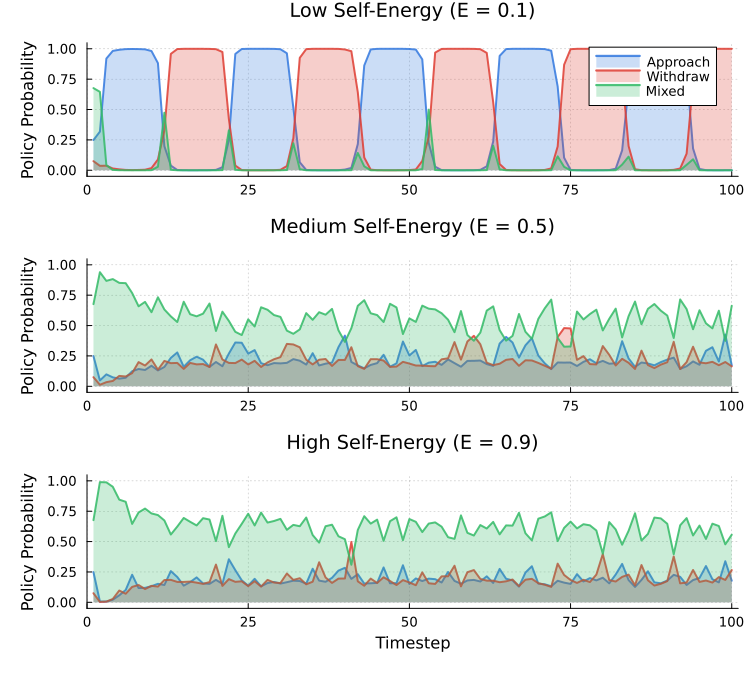
\includegraphics[width=0.92\linewidth]{polarization_policy.png}
\caption{Policy selection under polarization. The transition from takeover to coexistence proceeds through a higher-entropy exploration band.}
\label{fig:polarization-policy-v5}
\end{figure}
\FloatBarrier

\begin{figure}[H]
\centering
\includegraphics[width=0.92\linewidth]{polarization_summary.png}
\caption{Summary metrics for oscillation, switching, entropy, and simultaneous representation across polarization regimes.}
\label{fig:polarization-summary-v5}
\end{figure}
\FloatBarrier

\begin{figure}[H]
\centering
\includegraphics[width=0.92\linewidth]{polarization_combined.png}
\caption{Combined polarization figure showing the full transition from capture, to exploration, to negotiation as Self-energy rises.}
\label{fig:polarization-combined-v5}
\end{figure}
\FloatBarrier

The polarization simulation introduces two mutually threatening bundles:

\begin{itemize}
\tightlist
\item
  Part A: approach, disclose, attach
\item
  Part B: withdraw, protect, avoid
\end{itemize}

Under low Self-energy, the activations alternate in anti-phase. Each
bundle becomes locally true when active and intolerable when not. Under
high Self-energy, both remain representable together and a mixed policy
becomes possible.

The summary metrics suggest a three-regime picture:

\begin{itemize}
\tightlist
\item
  \textbf{Low Self-energy:} mutual takeover and narrow policy dominance
\item
  \textbf{Medium Self-energy:} exploration band with high entropy and
  switching
\item
  \textbf{High Self-energy:} stable simultaneous representation and
  reduced switching
\end{itemize}

That middle band is theoretically useful. It suggests that
de-polarization may not look like immediate calm. It may first look like
more simultaneous representability, more policy experimentation, and
only later like stable negotiation.

\begin{figure}
\centering
\pandocbounded{\includegraphics[keepaspectratio,alt={Figure: Polarization summary metrics}]{figures/polarization_summary.png}}
\caption{Figure: Polarization summary metrics}
\end{figure}

\emph{Figure B1. Polarization summary across Self-energy levels. Low
Self-energy produces anti-phase oscillation. Medium Self-energy
increases policy entropy and switching. High Self-energy produces the
most stable co-representation with the least switching --- suggesting a
three-regime transition from capture through exploration to
negotiation.}

\end{document}
